\documentclass[a4paper,10pt]{article}
\usepackage[english]{lsspub} % default is babel's ngerman
\usepackage{pgf}
\usepackage{physics}
\usepackage{amsmath}
\usepackage{amssymb}
\usepackage{amsfonts}
\usepackage{float}
\usepackage[parfill]{parskip}
\usepackage[ruled,vlined]{algorithm2e}
\usepackage{import}
\usepackage{todonotes}
\usepackage{tikz-uml}

\newtheorem{definition}{Definition}

% SETUP OF LSSPUB
\lsstitle{Optimization of Mirrorshapes in Optically Pumped Solar Lasers Using Ray Tracing Simulation Techniques}%
\lssauthor{Matthias König}%
\lsstype{Master's Thesis}%
\lssabstract{
\normalsize
This work showcases the application of ray tracing techniques for the calculation of absorption profiles in
optically pumped solar lasers.
It aims at using a lightweight and fast physically based raytracer combined with a biobjective
mesh adaptive direct search algorithm to optimize total power absorption and to minimize variance across the crystal.
An exemplatory setup of a side pumped Nd:Yag solar laser was simulated, optimized and the resulting
beam quality evaluated.
}

% CONDITIONALLY SET UP PDF-SPECIFIC STUFF (OPTIONAL)
\usepackage{ifpdf}

\ifpdf
% look at documentation for non-pdflatex setup of hyperref
\usepackage[pdftex]{hyperref}
\usepackage{natbib}
\hypersetup{colorlinks=true}
\hypersetup{linkcolor=black}
\hypersetup{citecolor=black}
\hypersetup{pdfauthor=\lsstheauthor}
\hypersetup{pdftitle=\lssthetitle}
\hypersetup{pdfsubject={\lssthetype, Informatik 10, Universität Erlangen-Nürnberg}}
\hypersetup{pdfkeywords={Solar Laser, Raytracing, MADS, Blackbox Optimization}}

% if you want thumbnails for your pdf, you need an additional
% call of thumbpdf and pdflatex after pdflatex converged 
% (i.e. all references were resolved etc.)
%
%\usepackage{thumbpdf}
%\hypersetup{pdfpagemode=UseThumbs}
\fi

% START LATEX DOCUMENT BODY

\renewcommand{\vec}[1]{\mathbf{#1}}
\newcommand{\equref}[1]{Eq.~(\ref{#1})}
\newcommand{\secref}[1]{Section~\ref{#1}}
\newcommand{\figref}[1]{Figure~\ref{#1}}
\newcommand{\algref}[1]{Algorithm~\ref{#1}}
\newcommand{\tabref}[1]{Table~\ref{#1}}
\newcommand{\defref}[1]{Definition~\ref{#1}}

\begin{document}

    % The following command creates the title page(s) and the text required
    % by the Pruefungsamt, stays German even if english option enabled
    % You can optionally provide a date for the signature line),
    % otherwise \today is used.
    \makelssthesis{Prof.~Dr.~C.~Pflaum}{1.11.2021 -- 2.5.2022}

    % Now the acutal thesis can start

    \tableofcontents

    \newpage

    \section{Introduction}

    In the light of the recent developements in global energy policy,
    renewable energy has become one of the most important
    problems humanity has to solve.
    Ever new ways of exploiting the sun's vast amount of energy are
    becoming relevant if nations across the world want to achieve
    net zero carbon emissions.
    One of those novel methods is the generation of hydrogen from
    water using solar energy.
    It can be achieved by common electrolysis or by reacting alkali
    metals with water.
    Researchers have been specifically looking at reacting magnesium
    ($Mg$) with water ($H_2O$) to produce hydrogen ($H_2$) and magnesium oxide
    ($MgO$)~\cite{solar_lasers_paper}.
    This reaction is exotherm and therefore causes a large amount of heat
    and produces hydrogen gas which could be stored in hydrogen fuel cells.
    Now if one can reduce the magnesium oxide to pure magnesium using
    the suns energy one would have a solution to store solar energy
    using hydrogen.
    To drive the reduction of magneisum oxide a laser can be used but
    a considerable amount if energy is needed.
    In order to reduce losses that are induced by using a conventional
    solar panel that drives a diode to pump the laser, it could be
    benefitial to pump the laser crystal directly using sunlight.
    This is exactly what Shigeaki Uchida and his team in Japan have
    been researching~\cite{solar_lasers_wiki}~\cite{solar_lasers_magnesium}.
    
    Another area of application that is becoming increasingly relevant is
    the usage of solar lasers in space exploration.
    Since there is no access to grid power in space and nuclear power
    is coupled with significant costs solar power is the most used
    source of power in space.
    The low efficiency of solar panels and the reduced number of parts
    of solar lasers make them an interesting prospect for usage in
    space.
    As mass is a high cost factor in space exploration the reduced weight
    and lower number of potential points of failure solar lasers could
    become a more relevant option in the future.
    The tasks of a solar laser in space could range from deep space
    communication, remote power transmission or tracking of objects.

    Solar lasers require the collection of sunlight and focusing
    onto a gain medium to surpass the lasing threshold thereof.
    As it is the most simple and cost effective method, usually
    a primary collector is used together with a secondary mirror in a 
    two stage collector to focus the sunlight onto the gain medium
    ~\cite{solar_lasers_magnesium}.
    The primary collector can be another mirror or a fresnel lens
    as a cheaper alternative.
    The beam power and quality is significantly impacted by the
    amount of power absorbed by the gain medium and the uniformity
    of the absorption profile.
    The natural divergence of sunlight and dispersion effects in the
    fresnel lens make it important that the secondary mirror is shaped
    in an optimal way.
    Both absorbed power and the uniformity of absorption need to be
    optimized.
    For the optical design of the collection system it is benefitial
    that the system is simulated accurately beforehand.
    For both the simulation and optimization part of the design process
    a free and open source framework was developed in this work in the
    hope that parts or the entirety of code may prove useful to engineers
    designing solar lasers.
    The goals of the framework are to offer a simple yet powerful interface
    for C++ applications.
    It provides a fast 2D raytracer for the calculation of the
    absorption profile in the gain medium which is then used by a
    mesh adaptive direct search algorithm in a biobjective manner (BIMADS) 
    to increase both absorbed power and uniformity of the absorption profile.
    This is done via the open source library NOMAD version 3~\cite{nomad3},
    which implements the MADS~\cite{mads_original} algorithm and a biobjective
    variant of it. 
    It offers the efficient derivative free optimization of a black-box
    function with constraints.

    The application of the framework is then demonstrated via an examplatory
    setup of a Nd:YAG solar laser using a two stage concentrator consisting
    of a fresnel lense and a secondary mirror.
    In principle, any parameter of the setup can be optimized but for this
    example in particular the mirrorshape is the interesting property. 
    The result of the BIMADS algorithm is a pareto front of optimal points 
    determined by the algortihm.
    Depending on whether a more even distribution of power is desired or
    the total amount of power absorbed is relevant to the application,
    some points of the pareto front are then chosen and simulated with
    the software ASLD~\cite{asld_website} to evaluate the resulting beam properties.

    \newpage

    \section{Lasers}

    Laser is an acronym which stands for \b{L}ight \b{A}mplification
    by \b{S}timulated \b{E}mission of \b{R}adiation.
    Lasers amplify coherent radiation at the infrared, visible, or
    ultraviolet part of the electromagnetic spectrum~\cite{lasers_siegman}.
    The principle was originally used in so called masers the 
    amplification of \b{M}icrowave radiation or even radio frequencies.
    The advantages of using a laser system as a lightsource are that
    they produce a directional beam of coherent light which can be 
    focused to a narrow spot~\cite{lasers_liverpool}.
    Additionally the emitted light is usually of a very narrow spectrum
    and thus reduces dispersion effects when shooting the beam through
    different media.
    Lasers are therefore used in a wide variety of applications which
    range from manufacturing processes to measuring systems to 
    optical communication.

    A laser usually consists of a gain medium that is capable of amplifying
    light that passes through by stimulated emission, a pumplight to
    excite the atoms of the gain medium to higher quantum states and
    an optical feedback mechanism - often called cavity or oscillator - 
    which usually
    consists of two mirrors that bounce the light back and forth through
    the gain medium~\cite{lasers_siegman}.
    One of those mirrors is only partially reflective and is transparent
    so that a portion of the amplified light can escape.
    Usually in more complex setups cooling is applied to the gain medium
    and some other optical elements like
    lenses or polarization filters may be present to ensure a better
    output beam quality.
    An ideal output beam is both temporally and spatially coherent,
    meaning that the emitted light is a perfect sine wave with constant
    amplitude und frequency and has a definite amplitude and phase pattern
    across any transverse plane inside the laser~\cite{lasers_siegman}.

    \subsection{Stimulated Emission}

    There are three ways in which atoms exchange energy with a radiation
    field~\cite{lasers_liverpool} identified by Albert Einstein.
    There is absorption where an electron is excited by a photon to a higher
    quantum energy state.
    Hereby the photon must have the exact amount of energy (wavelength)
    that the difference between energy state is.
    Then there is spontaneous emission where the excited electron jumps
    back to a lower energy state, emitting a photon in a random direction
    with a random phase shift
    but again with the same amount of energy as the difference between 
    states of the electron.
    This can occur spontaneously at any time as the name suggests. 
    The main priciple why the gain medium amplifies light is the priciple
    of stimulated emission.
    Electrons in the gain medium are stimlated by photons to a higher
    energy state.
    If now a again photon with the same amount of energy and a certain
    direction hits the atom the electron jumps back to the lower state
    again emitting a photon of the same energy but crucially and contrary
    to spontaneous emission in the exact same direction and the exact
    amount of phase shift as the incoming photon.
    Therefore amplifying the light by essentially "duplicating" the incoming
    photon.

    Now if one wants a coherent output beam one needs to make sure that
    the photons are travelling only in one direction and with constant
    phase.
    This is the job of the resonator.
    It uses the photons from spontaneous emission which at some point
    will have the correct direction and bounce them between the mirrors.
    Photons with other directions will be lost from the sides entirely
    or will get absorbed again by the medium.
    Due to this process a majority of photons will be travelling in the
    desired direction after some time.

    \subsection{Gain Medium and Population Inversion}

    In order to be able to amplify the emitted light, more atoms in the
    gain medium have to be in an already excited higher state than
    in the lower state.
    Otherwise "duplicated" photons will be reabsorbed by atoms in lower
    state and will not be able to stimulate another emmission or make
    it out of the laser cavity.
    Hence the population of atoms needs to be inverted~\cite{lasers_liverpool}.
    For this to happen an external source of energy needs to be supplied.
    This is called pumping and is usually achieved by a pump flash light
    or another laser.
    As it is equally likely that a photon causes stimulated emission or
    absorption there can not be only two states but at least three
    states are needed in optically pumped lasers~\cite{lasers_rpphotonics}.
    The electrons are then excited into the highest state by the pump
    light from which they can decay into the middle state ready for
    stimulated emission.
    It is crucial for level three lasers that the pump light cannot
    push the electrons in the middle state back to ground state.
    This way it is possible to have more atoms in the middle state than
    in ground state and therefore population inversion is achieved.
    For this to happen the pump light intensity in level three lasers
    needs to be sufficiently high enough for the photons to be "ignored"
    by the electrons in the second state.
    The threshold for the pump power to achieve population inversion
    is called the \emph{lasing threshold} and due to the
    energy levels in the atoms the choice of gain medium usually
    implies the choice of pump light or vice versa.  

    Materials that offer this property can be in gas, liquid or solid form.
    Solid form lasers are usually some sort of ion doped crystals or
    semiconductor diodes~\cite{lasers_liverpool}.
    As an example for a three level gain medium ruby ($Cr^{3+}:Al_2O_3$)
    can be used.
    In practice mostly four level gain media are used as they offer a 
    far lower lasing threshold for the pump power~\cite{lasers_rpphotonics}.
    These are usually neodymium doped media like the most popular choice
    neodymium doped yttrium aluminum garnets (Nd:YAG).

    \section{Raytracing Framework}
    With the advent of cheap processors and increasingly powerful 
    consumer hardware, ray tracing has become more popular in
    recent years.
    For the purpose of global illumination in video games and image
    processing, more advanced techniques have been continuously
    developed and improved.
    In optical design ray tracing is used to analyse the imaging 
    quality of optical systems or as in this work other 
    illumination properties can be simulated.
    The need for fast refresh rates in video games and the requirement
    of modelling more complex physical phenomena in optical design
    have led to tracing and sampling techniques that reduce the
    computational expense dramatically with minimal loss of accuracy. 
    Focused on the specific problems of laser design, these
    improvements make it possible to get physically accurate results
    in an acceptable amount of computational time in an iterative
    context.

    As in optical design systems are mostly rotationally symmetrical,
    the framework is meant to be used in a two dimensional setup
    and calculated quantities, e.g. absorbed power in a medium 
    converted to three dimensional values after a simulation step.
    This significantly reduces the amount of rays needed to avoid
    undersampling effects and to produce stable results across multiple
    simulation runs.
    Intersection tests also require less computation and objects in the
    scene require less fundamental shapes to test a ray against.
    The resulting performance gains makes it possible to run the 
    simulation thousands of times in an iterative process to 
    optimize some parameters in the optical setup even on consumer
    grade hardware.
    The objects in a scene are preproccessed to group fundamental shapes
    into leaves of a quadtree to reduce the amount of shapes a ray has
    to be tested against even further.
    To achieve the satisfied accuracy and to reduce noise the appropiate
    sampling strategies have to be used for a given problem.
    The most important techniques are provided including 
    uniform sampling, stratified and importance sampling.
    
    The framework was designed to provide a simple yet powerful
    interface for the user and was implemented in C++17.
    It provides the necessary data structures and algorithms for
    a fast raytracing solution.
    The sampling techniques are implemented in specialized classes
    of abstract interfaces. 
    They can also be used by the user to 
    implement custom techniques.
    The framework extensively relies on lambda functions to be
    provided by the user and thus naturally is customizable,
    although some preset functions are also provided.
    Because the calculations in the framework are so similar to applications
    in graphics software the OpenGL Mathematics header only library
    GLM~\cite{glm} was used as an underlying maths library.
    GLM is based on the OpenGL Shading Language (GLSL) and so in a 
    potential later step the framework
    could be ported to work on graphics cards providing that the
    data structures are changed to be accessable from a GPU.
    As in the specific problem in this work the tracing of each ray
    has side effects on the scene and on itself,
    i.e. the absorbed power of each ray has to be accumulated,
    it was decided to focus more on single core performance first
    and leave the parallel execution and execution on GPUs for a 
    later point.
    Furthermore IO utilities for simulations are provided for Comma 
    Separated Values (CSV) files and structured output for the 
    commonly used Visualization Toolkit (VTK)~\cite{vtk}.

    In the following chapters the applied ray tracing techniques 
    explained in detail.
    Firstly the basics of raytracing, i.e. intersection tests of
    fundamental shapes and objects and reflection and refraction effects
    are shown.
    Then an applied method of subdivision for the performance optimization
    of the raytracer is explained.
    Lastly some methods of sampling are shown before the structure of the 
    developed framework is presented with code samples.
    Here the usage of classes is demonstrated and it is shown how specific
    objects are defined.
    In particular the objects which are relevant for the simulation
    of laser cavities and which are used in the example setup are shown.

    \subsection{Raytracing Basics}  \label{sec:raytracing_basics}

    The techiques presented in this chapter are largely explained
    in the excellent lecture \emph{Global Illumination} by 
    Stamminger at FAU~\cite{globillum}.
    While the lecture applies those techniques in a different context,
    namely for the purpose of generating physically accurate images
    in image processing applications or video games,
    a selection of the techniques are still relevant to using
    ray tracing in scientific computing.
    Since the aim of both fields is slightly different, the priorities
    shift regarding to computational performance or numerical
    accuracy.
    In scientific computing more focus is layed on the accurate modelling
    of physical phenomena.
    For example, while in image processing it is sufficient to use a
    faster approximation of Snell's law in \equref{equ:snell} in application
    of physical rayracing one migt rather evaluate the actual law and
    take the additional computational cost of evaluating trigonometric
    functions into account.
    Nevertheless there is a large overlap between the two fields of
    application and a lot of techniques are entirely applicable
    in scientific computing as is.

    Rays are represented as a parametric line from a ray origin $o$ in
    direction $d$.
    The parameter $t$ goes is in the interval $[0, \infty)$ and represents
    the closeness of the ray to the origin.
    The mathematical representation therefore is given as

    \begin{equation}
        \label{equ:ray}
        \vec{r}(t) = \vec{o} + t\vec{d}
    \end{equation}

    After the ray is generated it is tested against intersections with the
    scene.
    Here the smallest $t > 0$ of all the intersections with objects has to
    be found.
    The question if a ray intersects an object can usually only be answered
    for simple fundamental shapes, e.g. lines, circles, axis aligned bounding
    boxes (AABBs) in 2D or planes, triangles, spheres, etc. in 3D.
    Therefore objects are normally comprised of a collection of fundamental
    shapes and an intersection occurs if one of the fundamental shapes is
    intersected.
    Naturally, an object can be intersected multiple times by the same ray
    and so the results have to be searched for the smallest $t$.
    Each fundamental shape should be represented in a parametrised form 
    so the intersection test can be represented as a system of equations.
    The two fundamental shapes used in this work are 2D lines and axis
    aligned bounding boxes (AABBs).

    Lines are represented by two points $\vec{a}$ and $\vec{b}$.
    So the intersection problem can be written as a ray-ray intersection
    as follows:

    Find $\alpha \in [0,1]$ and $t \in [0, \infty)]$ s.t. 

    \begin{equation}
        \label{equ:line_intersect}
        \vec{a} + \alpha (\vec{b} - \vec{a}) = \vec{o} + t \vec{d}
    \end{equation}

    If such a combination of $\alpha$ and $t$ exists, we have an intersection.
    As we are in 2D there are two equations for two unknowns and the
    system always has a solution.
    The solution can then be checked, s.t. the values are in the right
    intervals.
    A small mathematical trick is to define a 2D cross product which
    is basically just the $z$ component of a 3D cross product if the
    two input vectors $\vec{p}$ and $\vec{q}$ were parallel to the
    $xy$ plane:
    
    \begin{equation}
        \label{equ:2d_cross}
        \vec{p} \cross \vec{q} = 
        p_x \cdot q_y - p_y \cdot q_x \in \mathbb{R}
    \end{equation}

    Observe that same as the 3D cross product, the 2D version becomes 0
    when you cross a vector with itself.
    If one now crosses \equref{equ:line_intersect} with $\vec{d}$ on
    both sides the intersection equation becomes:
    
    \begin{equation}
        \label{equ:line_intersect_elim}
        \vec{a} \cross \vec{d} + \alpha (\vec{b} - \vec{a}) \cross \vec{d} =
        \vec{o} \cross \vec{d}
    \end{equation}

    So $t$ has been eliminated from the equation and we can solve 
    \equref{equ:line_intersect_elim} for $\alpha$:

    \begin{equation}
        \label{equ:line_intersect_alpha}
        \alpha = \frac{(\vec{a} - \vec{o}) \cross \vec{d}}
                      {\vec{d} \cross (\vec{b} - \vec{a})}
    \end{equation}

    If $\alpha$ satisfies the condition, we continue analogously for
    $t$ by crossing \equref{equ:line_intersect} with $\vec{b} - \vec{a}$.
    The resulting $t$ is then checked against the condition and
    a normal at the intersection point is calculated.
    The intersected rays can be seen in in \figref{fig:line_intersect}.

    \begin{center}
        \begin{figure}
            \centering    
            \def\svgwidth{0.8\textwidth}
            \import{images/}{line_intersect.pdf_tex}
            \caption{
                Ray-line intersection of two rays. The line is specified by
                the points $\vec{a}$ and $\vec{b}$ and the rays are 
                defined by
                the origins $\vec{o}_i$ and directions $\vec{d}_i$.
                Ray $(\vec{o}_1, \vec{d}_1)$ satisfies the conditions 
                $t \geq 0$ and $0 \leq \alpha \leq 1$
                and therefore causes an intersection, ray $(\vec{o}_2, \vec{d}_2)$
                dissatisfies the $\alpha$ condition and ray $(\vec{o}_3, \vec{d}_3)$
                does not satisfy the $t$ condition. 
            }
            \label{fig:line_intersect}
        \end{figure}
    \end{center}

    Another important shape to intersect are AABBs.
    They are rectangles aligned with the axis of the coordinate system
    so they require minimal memory space and intersection tests are
    as simple as possible.
    They most often used to surround complex objects or parts of it
    to reduce the amount of intersection tests.
    First the AABB of the object is tested and only if there is an
    intersection the actual fundamental shapes inside the AABB are tested.
    A 2D AABB is defined by two points $\vec{b}_{min}$ and $\vec{b}_{max}$ which
    represent the lower left and upper right corner of the rectangle.
    The intersection test is done by comparing the values of $t$ at each
    of the axis aligned lines defining the box.
    The $t$ values for the $x$ axis aligned lines can be calculated as
    shown in \algref{alg:aabb_intersect}.

    \begin{algorithm}
        \label{alg:aabb_intersect}
        \SetAlgoLined

        ${t_x}_1$ = $\frac{{b_{min}}_x - o_x}{d_x}$\;
        ${t_x}_2$ = $\frac{{b_{max}}_x - o_x}{d_x}$\;
        $t_{min}$ = $\min({t_x}_1, {t_x}_2)$\;
        $t_{max}$ = $\max({t_x}_1, {t_x}_2)$\;
        ${t_y}_1$ = $\frac{{b_{min}}_y - o_y}{d_y}$\;
        ${t_y}_2$ = $\frac{{b_{max}}_y - o_y}{d_y}$\;
        $t_{min}$ = $\max(t_{min}, \min({t_y}_1, {t_y}_2))$\;
        $t_{max}$ = $\min(t_{max}, \max({t_x}_1, {t_x}_2))$\;

        \If{$t_{min} \geq 0$ and $t_{min} \leq t_{max}$}{
            AABB was hit!
        }
        \caption{
        Intersection test for a AABB $(\vec{b}_{min}, \vec{b}_{max})$
        with ray $(\vec{o}, \vec{d})$
        }
    \end{algorithm}

    If the conditions $t_{min} \leq t_{max}$ and $t_{min} \geq 0$ hold
    there is an intersection.
    This process is better understood visually and is illustrated in 
    \figref{fig:aabb_intersect}.
    If normals are needed they can be easily calculated since there are
    only four possibilities depending on which side of the box is
    intersected first. 

    \begin{center}
        \begin{figure}
            \centering    
            \def\svgwidth{0.6\textwidth}
            \import{images/}{aabb_intersect.pdf_tex}
            \caption{
                Ray-AABB intersection, where first the intersection points with
                the $x$ axis (marked in green) and $y$ axis (marked in blue) are
                calculated.
                Each of the values ${t_i}_1, {t_i}_2$ are then split into the minimum
                and the maximum of the two.
                Both maximums are then compared and the minimum is chosen as the final 
                $t_{max}$.
                Analogously the minimums are compared and the maximum is chosen as
                $t_{min}$ (marked with red circles).
                Thus there is an intersection with an entry point 
                $\vec{o} + t_{min}\vec{d}$ and an exit point 
                $\vec{o} + t_{max}\vec{d}$ and the normals can be calculated depending
                on which sides the points reside.
            }
            \label{fig:aabb_intersect}
        \end{figure}
    \end{center}

    The AABB intersection becomes really handy once one wants to use them
    for ray tracing acceleration techniques, as they can easily be constructed
    to surround a cloud of points and then be used as a spacial subdivider
    in a tree structure.
    This is described in detail in the next chapter.
    Other shapes like circles or ellipses are intersected in a similar way
    but as they are not used in the example below the intersection process
    is not explained here.

    Once an intersection takes place, the ray will be either reflected, terminated
    or refraction occurs depending on the desired material of the object.
    Total reflection is only dependent on the incident angle $\theta_i$ 
    to the normal of the surface at the hitpoint.
    Then the reflection angle $\theta_r$ is given by \equref{equ:reflection}.

    \begin{equation}
        \label{equ:reflection}
        \theta_r = -\theta_i
    \end{equation}

    A new ray is then generated at the hitpoint pointing in the direction
    given by $\theta_r$.
    Due to limited floating point precision, it is required that the origin
    of the new ray is shifted by a small $\epsilon$ towards the 
    reflection direction in order to make sure the ray is originated at the
    correct side of the material.
    Since the reflection is total the entire amount of power of the incident
    ray is transferred to the reflected ray.

    When hitting a material that is transmissible for light the ray
    will be refracted at the boundary between the two media.
    The effects of matter on a light beam are described by Snell's law
    and the Fresnel equations.
    The ray is split into a reflected and a transmitted ray.
    The direction of the transmitted ray is governed by Snell's law in \equref{equ:snell}
    which depends on the indices of refraction of the two media $n_i$ and $n_t$.

    \begin{equation}
        \label{equ:snell}
        n_i \sin(\theta_i) = n_t \sin(\theta_t)
    \end{equation}

    Usually one rearranges the \equref{equ:snell} in order to solve
    for $\theta_t$.
    
    \begin{equation}
        \label{equ:snell_rearranged}
        \theta_t = \asin(\frac{n_i}{n_t} \sin(\theta_i))
    \end{equation}

    Arranged like in \equref{equ:snell_rearranged} one can observe
    that if $\frac{n_i}{n_t} > 1$ the argument of the $\asin$ function
    can also be greater than 1 depending on the incident angle
    $\theta_i$.
    In this case the arcussinus is undefined and therefore Snell's 
    law does not hold.
    But rather than presenting a mathematical problem this only
    models what happens in reality.
    If for instance a light ray transitions from a medium of higher
    refractive index $n_i$ to a medium woth lower refractive index
    $n_t$ and the angle of incidence $\theta_i$ is low enough
    for the expression $\frac{n_i}{n_t} \sin(\theta_i)$ to become
    greater than one, the light is no longer transmitted to the 
    medium wit lower refractive index.
    Instead the entirety of the light ray is reflected back to the
    medium with higher refractive index.
    This phenomenon is called total internal reflection and is an 
    effect that is abused in many physical applications, e.g.
    fiber optics communication.
    The light can travel along an optical fibre and even bends in the fibre
    because the material has high enoungh refractive index and the angle
    of light hitting the inside border from the fibre to air or other
    materials is low enough.
    In such scenarios the critical angle below which total internal reflection occurs is
    then given by ${\theta_i}_{crit} = \asin(\frac{n_t}{n_i})$. 
    An implementation of Snell's law therefore needs to detect, when
    total internal reflection takes place.
    Naturally, the reflected ray is still reflected as given in
    \equref{equ:reflection}.
    The transmitted and reflected power can be calculated with the transmission- and
    reflection rates given by Fresnel's equations.
    These are dependent on the orientation of the polarization of the incident ray
    (perpendicular or parallel) to the surface.

    \begin{equation}
        \label{equ:fresnel}
		R_{\perp} = \frac{\sin^2(\theta_1 - \theta_2)}{\sin^2(\theta_1 + \theta_2)} \quad
		R_{\parallel} = \frac{\tan^2(\theta_1 - \theta_2)}{\tan^2(\theta_1 + \theta_2)} \quad
		T_{\perp} = 1 - R_{\perp} \quad
		T_{\parallel} = 1 - R_{\parallel}
    \end{equation}

    For unpolarized light the total rates are just given by the average.
    
    \begin{equation}
        \label{equ:fresnel_unpolarized}
		R_{total} = \frac{R_{\perp} + R_{\parallel}}{2} \quad
		T_{total} = \frac{T_{\perp} + T_{\parallel}}{2}
    \end{equation}
    
    An additional effect that can be significant espacially for broadband
    applications is the dependency of the index of refraction of a medium
    on the wavelength of the light passing through and the dispersion
    of light resulting from this.
    This is modelled by the Sellmeier equation, which is based on 
    empirical measurements.
    The relationship between the refractive index $n$ and the wavelength 
    $\lambda$ in micrometers is described by a series of Sellmeier coefficients $B_i$ and
    $C_i$ that have been determined by experiment.
    The Sellmeier equation is thus given by \equref{equ:sellmeier}.

    \begin{equation}
        \label{equ:sellmeier}
        n^2(\lambda) = 1 + \sum_i \frac{B_i \lambda^2}{\lambda^2 - C_i}
    \end{equation}

    \subsection{Raytracing Acceleration} \label{sec:raytracing_acceleration}

    As the raytracer is later intended to be used in an iterative optimization
    algorithm, it is of vital importance that unnecessary computational cost 
    is avoided.
    For a raytracer this can be achieved in a number of ways.
    The first and simplest way is to simply reorder the objects in a scene
    by a heuristic that describes the likelihood of on object to be the
    first object hit by the majority of the rays.
    Of course, this only works well if rays are shot into a scene from
    a dominant direction.
    Another way would be to subdivide the entire 2D scene with quadtrees
    and try to fill each branch of the tree with an equal amount of 
    objects or shapes.
    
    Similarly one can also subdivide an object itself and sort the
    fundamental shapes comprising that object into a quadtree.
    This method was chosen in this work as there are a limited amount of
    objects in the scene with the objects possibly being quite complex.
    Once the fundamental shapes of an object are known, they can be
    sorted into a quadtree of AABBs of a chosen depth.
    The outermost AABB is the root of the tree with four children,
    each encompassing the shapes inside their quarter of space
    as tightly as possible.
    This is recursively done until the desired depth is hit.
    The intersection test of an object then can be done by hitting
    the root AABB of the tree and then stepping through its children
    via breadth first search.
    Each AABB child the ray hits, is persued further and the ones
    the ray doesn't intersect are ignored.
    If a leaf has been hit all the shapes inside are then tested for
    intersection.
    Finally the $t$ values of all the intersections are compared and
    the minimum and the maximum chosen as entry and exit points. 
    The advantage of this is that AABB intersection tests are done really
    fast and a large number of fundamental shape intersection tests
    are avoided.
    An illustration of subdivision of a mirror comprised of line segments
    is given in \figref{fig:quadtree} and a the intersecting algorithm
    for a single object is givin in \algref{alg:object_intersect}.

    \begin{center}
        \begin{figure}
            \centering    
            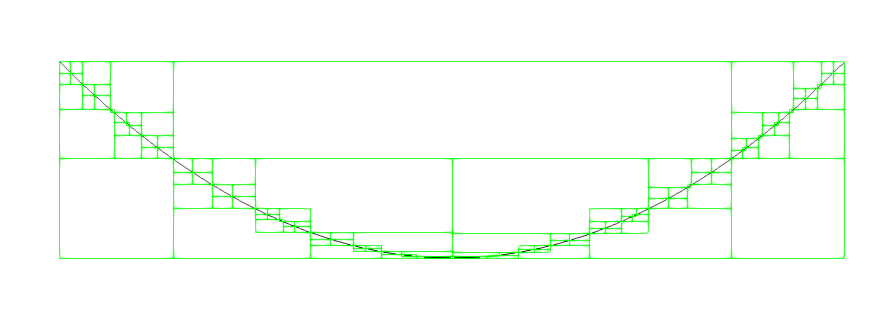
\includegraphics[width=0.8\textwidth]{images/mirror.png}
            \caption{
                A parabolic mirror comprised of line segments
                subdivided by a quadtree of AABBs with depth 4.
                Note that the AABBs are encompassing their contained line
                segments as tightly as possible.
            }
            \label{fig:quadtree}
        \end{figure}
    \end{center}

    \begin{algorithm}
        \label{alg:object_intersect}
        \SetAlgoLined
        IntersectionResult objectResult\;
        objectResult.tEnter = MaxFloatingPoint\;
        objectResult.tLeave = MinFloatingPoint\;

        Queue treeQueue\;
        treeQueue.push(object.root)\;

        \While{!treeQueue.empty()}{

            tree = treeQueue.front()\;
            IntersectionResult aabbResult = tree.aabb.intersect(ray)\;
            \If{aabbResult.hit}{
                \For{shapes in tree.shapes}{
                    IntersectionResult shapeResult = shape.intersect(ray)\;
                    \If{shapeResult.hit}{
                        set objectResult appropiately\;
                    }
                }
                treeQueue.push(tree.children)\;
            }
            treeQueue.pop()\;
        }

        \caption{Intersection test for a single object subdivided by a quadtree}
    \end{algorithm}


    \subsection{Sampling Techniques} \label{sec:sampling}

    The accuracy and performance of ray tracing simulations are heavily dependent upon
    using the correct sampling techniques.
    One could sample values on a uniform grid or equally spaced intervals.
    The problem with this is that there is no randomness or irregularity
    causing structured aliasing errors in most applications. 
    Random sampling however always relies on some sort of random number generation.
    These are usually pseudo random numbers generated according to some
    distribution with the generation engine initialized with a seed.
    Usually when one samples according to some scheme only values in 
    $[0,1]$ are allowed.
    The returned sample is then later scaled to the desired range depending
    on the usecase.
    It is also to be noted that calls to a sampler must be ensured to
    be as effiecient as possible as a large number of calls will be
    made during the simulation.

    The simplest sampling scheme is uniform sampling.
    It returns values uniformly and can be implemented right on top of
    the random number engine of the used system.
    The advantage of uniform sampling is that it produces close to random
    samples without the need for additional logic and therefore
    performance losses.
    The disadvantage is the irregular density of samples within the interval.
    There can be areas with a lot of samples and large gaps between.
    So in scenarios where there needs to be a more regular distribution
    of samples uniform sampling is not optimal.

    For this reason another sampling technique called stratified uniform
    sampling exists.
    Here the domain is split into $N$ equally spaced intervals and the
    uniform sampling occurs within each interval.
    This ensures that there is some amount of regularity while still
    keeping the randomness of uniform sampling.
    An application of stratified sampling would be the definition of
    a light source in the simulation.
    The direction or origin of the rays the light source emitts can be
    sampled according to stratified sampling to ensure a smooth
    illumination of the scene.
    The difference between uniform and stratified uniform sampling can
    be observed in \figref{fig:uniform_vs_stratified}.

    \begin{center}
        \begin{figure}
            \centering    
            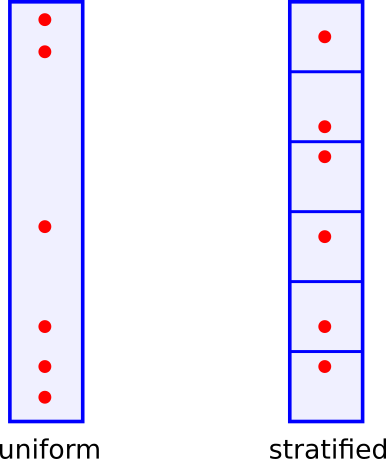
\includegraphics[width=0.25\textwidth]{images/stratified.png}
            \caption{
                Uniform sampling of a 1D interval (left) vs. stratified sampling (right).
                Observe the large gap between samples on the left whereas
                the samples on the right are spaced out more equally.
            }
            \label{fig:uniform_vs_stratified}
        \end{figure}
    \end{center}

    A more advanced technique is to sample values where they are contributing
    the most.
    Suppose one wants to approximate some function $f$ over a domain
    $[0,1]$.
    The criterium that has to be met in order to calculate some quantity
    $Q$ is given by any arbitrary integral in the domain.
    With uniform sampling of $x \in [x_1,x_2]$ by the sequence 
    $(x_i)$ and $i = 1...n$ the integral is approximated
    by \equref{equ:impsampling_uniform}.

    \begin{equation}
        \label{equ:impsampling_uniform}
        Q = \int_{x_1}^{x_2} f(x) dx \approx \frac{1}{n} \sum_{i = 1...n} f(x_i)
    \end{equation}

    Now it is also possible to sample according to some other distribution.
    One just has to know the probability density function (pdf) $p$ to know
    how likely it is that a sample $x_i$ is generated.
    Probability density functions are nonnegative across the domain
    and their integral over the domain is always 1.
    This corresponds to the probability that a sampled value is in the
    interval $[x_1, x_2]$ which is of course the case when all
    possible values are within that interval. 
    The more accurately the pdf $p$ matches $f$ the more $[x_1,x_2]$
    is sampled at the points where the function $f$ has a large contribution to
    the integral.
    This can significantly reduce the amount of samples needed to get an
    accurate approximation for the integral $Q$.
    The integral is then approximated by \equref{equ:impsampling}.

    \begin{equation}
        \label{equ:impsampling}
        Q = \int_{x_1}^{x_2} f(x) dx \approx \frac{1}{n} \sum_{i = 1...n} \frac{f(x_i)}{p(x_i)}
    \end{equation}

    Observe that now the values for $f$ are weighted by the likelihood $p$.
    If it is likely that a sample $x_i$ is generated - larger $p$ - then
    the contribution is worth less and vice versa.     
    Of course this requires some preprocessing in order to generate the
    distribution $P$ from a pdf $p$.
    Usually one wants to generate $p$ from $f$ but there are also 
    cases where one might choose another function to deduce the
    pdf and subsequently the distribution.

    One method of building such a distribution is to first integrate
    $f$ in the domain $[x_1, x_2]$ and normalize the function so the
    integral is guaranteed to be 1.
    Then to sample according to the resulting pdf one discretizes the
    pdf to a finite amount of equidistant intervals $p_i = [{x_1}_i, {x_2}_i]$.
    For an interval $p_j$ the values $p({x_2}_i)$ for all $i < j$ are
    then summed up progressively assigned to that interval.
    These resulting rectangles are then stacked so that each rectangle
    represents an interval in $x$ and the corresponding values of the
    sum of the pdf.
    Then a sample $\xi \in [0,1]$ is drawn from a uniform sampler and
    the corresponding interval in which the value $\xi$ lies in is
    searched in the list of intervals using binary search.
    Once the interval is found we interpolate linearly between the
    lower boundary ${x_1}_i$ and ${x_2}_i$ depending on $\xi$.
    Then the resulting $x \in [{x_1}_i, {x_2}_i]$ is returned along
    the value of the pdf $p(x)$ as a sample.
    This process approximates the distribution $P$ and is called the
    inversion method. It is better understood when visualized as in
    \figref{fig:impsampling}. 
    
    \begin{center}
        \begin{figure}
            \centering    
            \begin{tabular}{c c}
            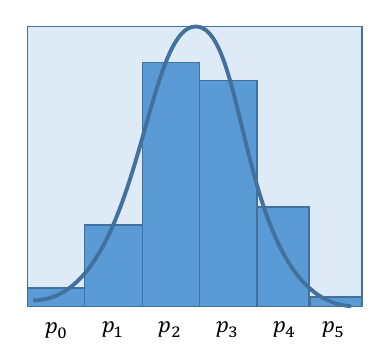
\includegraphics[width=0.3\textwidth]{images/impsampling_rectangles.png} &
            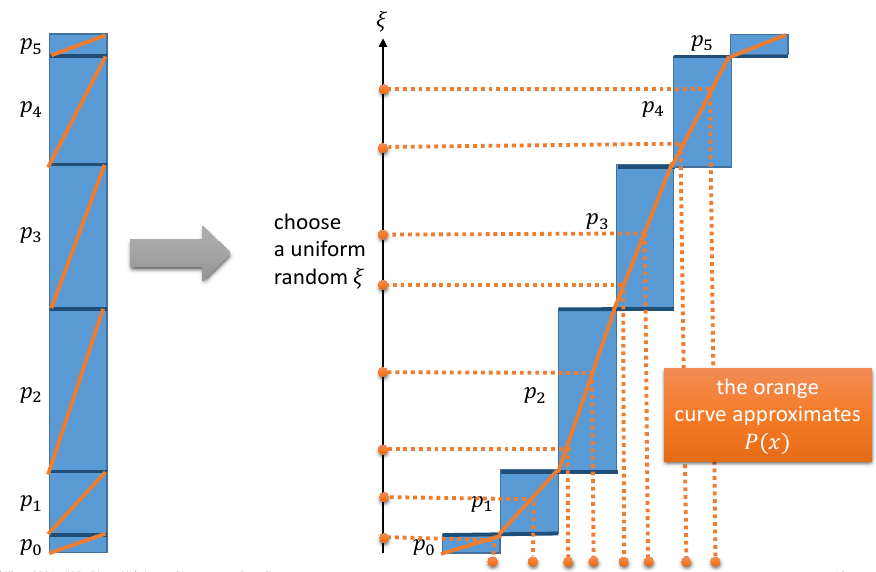
\includegraphics[width=0.7\textwidth]{images/inversion.png}
            \end{tabular}
            \caption{
                Visualization of inversion method to sample according the
                pdf on the left.
                The intevals $p_i$ are summed up and stacked.
                Then a $\xi \in [0,1]$ is uniformly sampled and the corresponding
                interval is searched.
                The returned value is interpolated linearly according to the value
                of $/xi$ within the rectangle.
            }
            \label{fig:impsampling}
        \end{figure}
    \end{center}
    
    \subsection{Framework Structure}

    The goal of the raytracing framework is to offer a free and lightweight
    alternative to commercial raytracers in order to stay efficient
    for the later usage in a black-box optimization context.
    For the optimization, it is crucial that the raytracer can be executed thousands of times
    even with a higher number of rays without significant overhead.
    It is to be noted that the raytracer has been specifically designed in
    order to be used in the optimization of geometrical parameters in
    rotationally symmetrical systems.
    Therefore the decision was made to work in a 2D context rather than a 3D
    one.
    The additional computational cost of going from a 2D to a 3D context for
    raytracing is significant and since the framework is to be used as
    the optimization part of the design process the results can then be
    taken and further analysed in a 3D raytracer.
    Suppose a 2D raytracer needs $10000$ rays to reduce the noise to a
    satisfactory level.
    Then it can be assumed that a 3D raytracer needs about $10000 \cdot
    10000$ rays to produce the same result.
    The only difference is that transversal rays cannot be modelled in
    2D but transveral rays which may occur by divergence of sunlight or
    scattering effects in inpure media are statistically distributed
    equally across the full rotation of a rotationally symmetrical system and the impact
    on the result is therefore negligable.
    Additionally, the described objects in the scene require a significantly
    higher amount of fundamental shapes, which compounds the performance
    loss of needing more rays even further.
    Furthermore the ray intersect equations shown above would become more
    complex and would require more arithmetic and cases.
    So for the relatively small benefit of being able to model transversal
    rays it is infeasable in a rotationally symmetrical system to simulate in a 3D environment.
    Of course, if the system is not rotationally symmetrical then there
    is no other choice than to trace the scene in 3D, but this is
    not the norm in laser optical systems.
    In the following chapter the most important parts of the raytracer
    framework are presented.
    The datastructures and algortihms are shown in an UML class diagram
    and an example application of the datastructure or algorithm is given. 
    It is to be noted that not all fields, methods or datatypes
    are shown in the UML diagrams and the code should therefore
    be seen as pseudocode instead of specific C++ code.
    When the classes have already been explained and the fields
    are not necessary to understand the relation between them
    they are omitted from the diagram to keep the diagrams more
    managable.
    The \emph{float} datatype represents some floating point datatype
    and not necessarily the C++ datatype.
    The \emph{vec*} vector datatypes are either the GLM~\cite{glm} datatypes
    for vectors - if the dimension is 4 or below - or a custom implementation
    to mimic the vector arithmetic of GLM for higher dimensions.
    Pointer datatypes in the UML diagrams are entirely reliant on
    the STL smart pointers in C++.
    Thus the user usually constructs instances of the objects or shapes
    via smart pointers which implement reference counting
    in order to manage heap allocated resources.
    Therefore there is no need for the user to worry about 
    memory management. 

    \subsubsection{Rays}

    Rays are the most basic datastructure in the simulation.
    They are described by an origin, a direction, a field for the
    amount of power, wavelength and a bool field if a ray has
    already been terminated.
    The simplest action is to just terminate the ray at some $t$
    in which case it will no longer be considered in the tracing
    algorithm.
    Rays can alse be reflected at a point $t$ with a certain normal, 
    where the original ray is terminated and a new ray according to \equref{equ:reflection} with a small
    $\epsilon$ shift for te origin in the reflected direction is returned.
    Another action is to refract the ray between the boundary
    of two media with refractive indices $n_1$ and $n_2$.
    Here a tuple of new rays is returned and the original ray
    is terminated.
    The first element is the reflected ray and the second
    element is the transmitted ray into the medium.
    The direction of the transmitted ray is calculated using
    \equref{equ:snell}.
    It should be noted here that as explained in
    \secref{sec:raytracing_basics}
    there does not necessarily exist a transmitted part of the ray.
    This is due to the phenomenon of total internal reflection
    which can occur once the ray transitions from a medium with high
    reflective index to a medium with low refractive index.
    In such cases the implementation of the \emph{refract} method
    detects that Snell's law is undefined and reflects the ray
    with the entire amount of power back into the medium.
    In the normal case the power of the original ray
    is split between the reflected and transmitted part according
    to the Fresnel laws \equref{equ:fresnel} for unpolarized
    light \equref{equ:fresnel_unpolarized}. 
    The UML class diagram for the Ray2D class and other relevant
    classes is shown in \figref{fig:uml_ray2d}.

    \begin{center}
    \begin{figure}
    \centering
    \begin{tikzpicture}
    \umlclass[]{Ray2D}{
      + origin : vec2 \\
      + direction : vec2 \\
      + power : float \\
      + wavelength : float \\
      + terminated : bool \\
      + terminatedAt : float
    }{
      + terminate(t : float) : void \\
      + reflect(t : float, normal : vec2) : Ray2D \\
      + refract(t : float, normal : vec2, n\_1 : float, n\_2 : float) : tuple<Ray2D, Ray2D> \\
    }    
    \end{tikzpicture}
    \caption{UML class diagram of the Ray2D class}
    \label{fig:uml_ray2d}
    \end{figure}
    \end{center}

    As the user rarely has to interact directly with ray class and
    the implementation and usage of the methods are straight forward
    an example is not necessary here.
    
    \subsubsection{Shapes}

    The Shape2D class represents all fundamental shapes in two dimensions
    It is the baseclass for all specific 2D shapes like lines, AABBs or circles
    etc.
    The specific intersection tests with rays are implemented in those derived
    classes.
    Each shape additionally has an AABB that encompasses the represented
    shape.
    This AABB is then used to construct the quadtree for the object the shape
    is part of.
    When a shape is intersected an interection result is returned, which
    contains the enter and leave $t$ value of the intersection and a boolean
    that represents whether an intersection has even occurred.
    Furthermore the normals at the enter and leave point are contained
    in the intersection result.
    Each shape also has a line representation in order to later output
    the scene in the VTK format for visualization.
    A UML class diagram of the Shape2D class is shown in 
    \figref{fig:uml_shape2d}.


    \begin{center}
    \begin{figure}
    \centering
    \begin{tikzpicture}
    \umlclass[x=-4, y=4]{IntersectResult2D}{
        + tEnter : float \\
        + tLeave : float \\
        + hit : bool = false \\
        + normalEnter : vec2 \\
        + normalLeave : vec2 \\
    }{}
    \umlclass[x=4, y=4]{AABB2D}{
        + bmin : vec2 \\
        + bmax : vec2 \\
        + hit : bool = false \\
        + normalEnter : vec2 \\
        + normalLeave : vec2 \\
    }{
        + getMidPoint() : float \\
        + isInside(vec2 point) : bool \\
    }
    \umlclass[type=interface]{Shape2D}{
    }{
      \umlvirt{+ intersect(ray : Ray2D) : IntersectResult2D} \\
      \umlvirt{+ lineRepresentation() : vector<vec4>}\\
    }
    \umlclass[x=-4, y=-5]{Line2D}{
      + a : vec2 \\
      + b : vec2 \\
    }{
      + Line2D(a : vec2, b : vec2) \\
      + intersect(ray : Ray2D) : IntersectResult2D \\
      + lineRepresentation() : vector<vec4>\\
    }
    \umlclass[x=0, y=-10]{BoundingBox2D}{
    }{
      + BoundingBox2D(bmin : vec2, bmax : vec2) \\
      + BoundingBox2D(points : vector<vec2>) \\
      + BoundingBox2D(aabb : AABB2D) \\
      + BoundingBox2D(aabbs : vector<AABB2D>) \\
      + BoundingBox2D(aabbs : vector<BoundingBox2D>) \\
      + intersect(ray : Ray2D) : IntersectResult2D \\
      + intersectCheck(ray : Ray2D) : IntersectResult2D \\
      + lineRepresentation() : vector<vec4>\\
    }  
    \umlclass[x=4, y=-5]{Sphere2D}{
      + center : vec2 \\
      + radius : vec2 \\
    }{
      + Sphere2D(center : vec2, radius : vec2) \\
      + intersect(ray : Ray2D) : IntersectResult2D \\
      + lineRepresentation() : vector<vec4>\\
    }  

    \umlimpl[geometry=|-]{Line2D}{Shape2D}
    \umlimpl[geometry=--]{BoundingBox2D}{Shape2D}
    \umlimpl[geometry=|-]{Sphere2D}{Shape2D}
    \umluniassoc[anchor1=70,arg=has,mult=1, geometry=|-]{Shape2D}{AABB2D}
    \umldep[anchor1=110, geometry=|-]{Shape2D}{IntersectResult2D}

    \end{tikzpicture}
    \caption{UML class diagram of the Shape2D and associated classes}
    \label{fig:uml_shape2d}
    \end{figure}
    \end{center}

    The shapes that are derived from the Shape2D class are the basic unit
    for the intersection tests used in the tracing algorithm.
    The implementation of those tests should therefore be computationally
    efficient and should avoid unnecessary branches.
    Ideally they should be branchless implementations where only the
    final decision if an intersection has occurred requires a branch.
    An example for a branchless intersection test has been shown
    in \secref{sec:raytracing_basics} above, specifically the ray-AABB
    and ray-line intersections.
    For the ray-AABB intersection two versions of the test should exist.
    One version that only checks for the intersection and one version,
    which also calculates the normals.
    The check-only variant should then be used in 
    \algref{alg:object_intersect}
    as no normals are needed to traverse the quadtree and
    the AABB normal calculation is quite branch heavy.
    This is what the \emph{intersectCheck} method of the BoundingBox2D
    class is for.
    Furthermore the BoundingBox2D class provides multiple ways of constructing
    the represented AABB.
    Either directly by giving $b_{min}$ and $b_{max}$ or by providing a point
    cloud or by merging multiple AABBs together.
    This is then later used in the construction of the quadtree of the object
    the shape is in.

    \subsubsection{Objects}

    Objects are represented by the Object2D class and are essentially a collection of
    Shape2D instances. 
    Similarly to the Shape2D class the Object2D is just the base class
    for the specific objects implemeted by the user or predefined by
    the framework.
    To initialize an object a list of shapes has to be provided.
    The constructor of the Object2D class then builds the quadtree
    of shapes from that list as described in 
    \secref{sec:raytracing_acceleration}.
    The intersection test for the object is then done as shown in
    \algref{alg:object_intersect}.
    Furthermore the object base class provides a virtual method 
    for a user defined action to be executed once a ray hits the
    object.
    A few presets are already implemented namely pass, absorb and reflect.
    Pass just ignores the object entirely, absorb terminates the ray at the
    entry point of the intersection and reflect reflects the ray at the
    hitpoint.
    The user defined action provides the capability for the framework to
    be extensible and customizable.
    It provides the ray, the intersection result and a reference to a
    list of newly created rays for the user.
    For example, the ray could hit the surface and spawn multiple
    new rays instead of just being reflected modelling
    some sort of scattering effect.
    This isn't implemented by the framework out of the box but
    the user can easliy implement this functionality in a single
    function.
    The Object2D class therefore is intended to provide the bare bones
    functionality for efficient tracing of an object, but the
    actual physical modelling of the interaction of a light ray
    with the object can be entirely customized by the user.

    Objects that are arbitrarily complex can thus be efficiently
    implemented with minimal programming.
    Examples of how the usage of the Object2D class is intended can
    be seen in the paragraphs below.
    Here a thin lense approximation, a reflective mirror, and a grid
    representing a laser crystal are implemented and can be used by
    the user.
    A UML class diagram of the Object2D class and associated
    classes is given in \figref{fig:uml_object2d}.

    \paragraph{Medium2D}
    All object that consist of some material that is transmissible by
    light and have a non negligable thickness should implement the
    Medium2D interface.
    It holds information about the material via the materials
    Sellmeier coefficients and implements the all the phenomena
    relevant to the correct tracing of light on the border
    between two materials of different refractive index. 
    These are Snell's law in \equref{equ:snell} for the bending of the ray on material
    boundaries, the Fresnel laws in \equref{equ:fresnel} for the
    correct amount of intensity to be transmitted or reflected and
    the Sellmeier equation of the lens material in \equref{equ:sellmeier}
    to accurately describe dispersion effects of the material.

    Like all objects in the simulation it inherits from the 
    Object2D class and implements the \emph{action} method in to
    include the above described effects.
    Furthermore the Medium2D class provides the abstract \emph{actionEnter}
    and \emph{actionTransmit} methods which are executed
    once the ray first hits the medium and once the transmitted part
    of the ray was traced within the medium respectively.
    They can then be implemented by the user in a user defined object
    implementing the Medium2D interface.
    These actions can even modify the affected light ray in order
    to model absorption or thermal lensing effects within the medium.
    If the ray is terminated by the user in the \emph{actionTransmit}
    function, no further tracing is done and no additional rays
    are created.
    An example of this modification to the ray itself by the user
    is the Grid2D class.
    Here the power of the ray is modified by each cell the ray intersects 
    in order to model the absorption of light within a medium.

    The Medium2D inteface should serve as the base class for all
    user defined objects where the tracing of light needs to
    be physically accurate.
    This means that no approximations are made and the required
    computation per ray transmitting through these objects is quite
    high.
    Additionally, one ray that hits the object then in turn creates
    three rays only one of which - the ray within the medium - is always
    guaranteed to be terminated.
    The other two generated rays, namely the reflected part and the
    ray exiting the medium on the other side are two completely
    new rays entering the scene.
    These rays then need to be traced, increasing the overhead
    of tracing a medium accurately even more.
    Therefore it is advised to use the Medium2D interface with
    great care and sparingly in order to keep the computational
    cost to a minimum.
    Only the most relevant objects to the simulation should be
    traced with full physical accuracy.
    Suppose one wants to model a mirror using the Medium2D class.
    Technically this is possible, but practically it is infeasable,
    since the only thing the user is most likely interested in
    is the reflected part of the incoming ray.
    The same is true for lenses or optical elements where either
    the dispersion effects are negligable or the angle of
    incidence is such that almost all light is transmitted
    anyway.
    In this case the user is most likely only interested in the
    transmitted part of the ray and not the reflected or internal
    part.
    To prevent this unnecessary computational cost, one usually
    wants to approximate or neglect certain parts of the
    tracing in media.
    This is what the ThinLens2D and Mirror2D classes shown below
    demonstrate.

    \paragraph{ThinLens2D}

    The accurate physical simulation of a lens follows the same laws
    as the ray tracing in all media.
    This is modelled by the Medium2D interface, which implement all
    relevant effects in a transmissible material.
    Although it is phyysically accurate to trace the light rays with
    the Medium2D class, significant amounts of computation is needed
    to calculate and describe the light paths.
    Furthermore, the geometry of the lens needs to be modelled accurately.
    This is simple for conventional glass lenses where the geometry can be
    described only by the radii of the surfaces and the thickness of the lens.
    But for fresnel lenses this process can be quite complex and time
    consuming, both in the modelling phase and the computational cost
    of tracing many fundamental shapes.
    Thus it is rarely feasable to trace lenses without any amount
    of simplification.
    The question of choosing the appropiate amount of approximation depends on the goal of the
    simulation and the use case of the optical system and cannot be
    generally answered.
    It can be required to trace a specific lens with all the effects described
    above if the goal of the simulation is to design that specific lens
    for example.
    For imaging systems like camera objectives, the lenses are usually
    aligned in their optical axis, rays are predominantly 
    entering the system at shallow angles and dispersion effects can 
    be largely neglected.
    Other tasks my require rays to hit the lens at odd angles so the
    correct geometry of refraction is important, but dispersion effects
    and transmitted power are not that important or can be 
    approximated by another way.
    Therefore the user ultimately needs to decide which amount of 
    approximation is acceptable for the task at hand.        

    Suppose the user simulates a camera objective.
    Like in most optical systems a larger number of lenses are 
    aligned in their optical axis and rays are only hitting the lens
    with a small angle with respect to those axis.
    Here the only thing that matters is the correct refraction of
    rays according to the rules of geometric ray tracing in a thin lens.
    Parallel rays always intersect the focal point and rays that
    travel through the middle of the lens will not be refracted
    at all.
    Those lenses are therefore often modelled by the ABCD ray transfer
    matrix~\cite{abcd_lens_rpphotonics}.
    The lens is seen as a sort of blackbox with a certain thickness
    and the transfer matrix describes how a ray is transmitted
    through the lens.
    The only information needed is the thickness of the lens and
    the focal point of the lens.
    If multiple lenses are in a row and described by ABCD transfer matrices,
    the transfer matrix of the whole system can then be calculated
    from the individual ones.
    The ABCD transfer matrix only provides correct results once the
    angles of the ray with respect to the optical axis of the lens
    are shallow.
    Then the $\sin(\theta)$ in Snell's law \equref{equ:snell} is
    just approximated by $\theta$ for small angles (paraxial approximation).

    Since lenses in the raytracer in this work can be rotated in any way,
    a more general approach is to solve a trigonometrical formula for
    each ray hitting the lens.
    In this case also rays with steep angles are refracted correctly.
    For the purposes of simplification the lens is usually made 
    infinitely thin.
    This way of tracing a thin lens is described in~\cite{thin_lens}.
    It provides a good compromise between an approximation and using 
    fully accurate refraction on a exactly modelled piece of glass, where normals and angles need to
    be calculated and the laws of Snell, Fresnel and Sellmeier need to be applied.
    Naturally, dispersion effects can not be modelled by this approach,
    but for non-imaging systems it is often sufficient to trace lenses
    without dispersion effects, especially because glass has a very
    low dependency of the refractive index on wavelength according to
    its Sellmeier coefficients.
    If one still wants to model dispersion effects with this approach,
    one method could be to provide an artificial thickness function 
    or just upper bound depending on the applications requirement for
    physical accuracy.
    Then the Sellmeier coefficients for the desired material of the lens
    in combination with the sampled thickness at the hitpoint can be used
    to disperse the ray correctly.
    An example for this would be a fresnel lens made from PMMA.
    The sawtooth pattern of the ridges could then be given as a function
    to be sampled at the hitpoint.

    The ThinLens2D class represents the approximation of a thin lens
    according to~\cite{thin_lens}.
    It takes the radius and desired focal length and constructs
    an object whose only fundamental shape is a Line2D shape representing
    the thin lens.
    Once a ray hits the line the ray is terminated and a new ray pointing
    in the direction of refraction is generated at the hitpoint.

    \paragraph{Mirror2D}

    Mirrors like lenses are commonly used in optical systems.
    Most of the time one wants optimize the shape of a mirror system
    in order to fullfill some optical property.
    As all objects in the framework, mirrors are also considered to be
    rotationally symmetrical.
    The mirrors implemented in the Mirror2D class consist of line segments
    of the class Line2D, the amount of which can be given as an argument
    to the constructor.
    Additionally the shape of the mirror can be given as a parametrized
    2D curve.
    The function should take a single parameter $t \in [0, 1]$ and return
    2D points along the curve.
    The parameters of the shape function can then be changed by the simulation
    in an optimization algorithm and the mirror reconstructed with the
    updated values using the \emph{rebuild} method.
    Naturally the action of the Mirror2D object is to reflect the ray
    according to \equref{equ:reflection}.
    
    \paragraph{Grid2D}

    The Grid2D class offers to simulate quantities distributed within
    a medium.
    Rays are traced according to the laws in \equref{equ:snell},
    \equref{equ:fresnel} and \equref{equ:sellmeier}.
    When the ray first hits the medium a hit action can be given if
    the hitpoint contains relevant information to the user.
    Then the distance within each cell the ray is travelling through
    is eveluated.
    It is to be noted that it is assumed the medium is homogenous and
    has constant refractive index.
    Thus the rays travel in a straight line within the medium.
    Additionally to the hit action a cell action can be given as a
    parameter to the constructor.
    The cell action function is executed once the ray hits a cell.
    The distance travelled through the cell is evaluated and given to the
    cell action function, which then in turn can access the cell
    values in order to change them.
    The tracing within the grid is done using a fast 2D voxel algorithm
    shown in ~\cite{voxel}.
    Here the cells are accessed in order the ray traverses them, which
    is important should the cell action change the ray parameters in
    any way.
    
    Absorbing media are modelled using the Grid2D class and
    supplying a cell action that evaluates the lost power via
    Lambert's law of absorption.
    It describes the exponential decay of the remaining power
    of a ray of light in an absorbing medium depending on
    the coefficient of absorption of the medium and the 
    distance travelled.
    The remaining power of a ray of light is then given by
    \equref{equ:lambert}.

    \begin{equation}
    \label{equ:lambert}
        P_{rem} = P_{ray} \cdot e^{-\alpha(\lambda) d}
    \end{equation}

    Here the absorption coefficient is $\alpha$ and the distance
    travelled by the ray is $d$. 
    In general $\alpha$ depends on the vacuum wavelength of the ray
    $\lambda$.
    For this reason an absorption spectrum of the medium can be supplied
    and evaluated at each cell.
    Since the ray's wavelength stays constant this evaluation can be
    optimized by evaluating $\alpha(\lambda)$ only once the ray hits the
    medium and keeping track of this value for successor cells.
    The absorbed power is then added to the cells value.
    Thus after a full simulation of the scene the absorbption profile
    is known.
    Additionally the total irradiation is evaluated when the ray hits
    the medium, if the user requires this information.
    Supplying the apsorption spectrum can be done by using the various
    utilities the framework provides.
    These are described in \secref{sec:utilities}.

    \begin{center}
    \begin{figure}
    \centering
    \begin{tikzpicture}
    \umlsimpleclass[x=5, y=5]{Shape2D}
    \umlclass[x=0, y=5]{Object2D :: Tree}{
        + box : BoundingBox2D* \\
        + children : vector<Tree*> children \\
    }{
        ...
    }
    \umlinterface[x=0, y=0]{Object2D}{
        \# subdivisions : uint \\
        \# pos : vec2 \\
        \# up : vec2 \\
        \# scale : vec2 \\
    }{
        + Object2D(shapes : vector<Shape2D*>, subdivisions : uint) \\
        + init() : void \\
        + intersect(ray : Ray2D) : IntersectResult2D \\
        \umlvirt{+ build() : void} \\
        \umlvirt{+ action(ray : Ray2D, result : IntersectResult2D, createdRays : vector<Ray2D>*) : void} \\
        ...
    }
    \umlclass[x=-4, y=-5]{Mirror2D}{
        - shapeFunction : function<vec2(float)> \\
        - segments : int \\
        ...
    }{
        + action(...) : void \\
        ...
    }
    \umlclass[x=4, y=-5]{ThinLens2D}{
        - radius : float \\
        - focalLength : float \\
    }{
        + action(...) : void \\
        ...
    }
    \umlinterface[x=0, y=-9]{Medium2D}{
       \# sellmeierCoeff : vec4; 
    }
    {
        + action(...) : void \\
        \umlvirt{+ build() : void} \\
        \umlvirt{+ actionEnter(ray : Ray2D, result : IntersectResult2D) : void} \\
        \umlvirt{+ actionTransmit(ray : Ray2D, result : IntersectResult2D) : void} \\
        ...
    }
    \umlclass[x=0, y=-14.5]{Grid2D}{
        - bmin, bmax : vec2 \\
        - maxX, maxY : int \\
        - data : vector<float> \\
        - cellAction : function<void(ray : Ray2D, distance : float, cell : float*)> \\
        - hitAction : function<void(ray : Ray2D, result : IntersectionResult2D)> \\
        ...
    }{
        + sum() : float \\
        + avg() : float \\
        + var() : float \\
        + stddev() : float \\
        + reset() : void \\
        ...
    }

    \umluniassoc[arg=has, mult=1, geometry=--]{Object2D}{Object2D :: Tree}
    \umlimpl{Mirror2D}{Object2D}
    \umlimpl{ThinLens2D}{Object2D}
    \umlinherit{Medium2D}{Object2D}
    \umlimpl{Grid2D}{Medium2D}
    \umlunicompo{Object2D :: Tree}{Shape2D}

    \end{tikzpicture}
    \caption{UML class diagram of the Object2D and associated classes}
    \label{fig:uml_object2d}
    \end{figure}
    \end{center}

    \subsubsection{Scene}

    The Scene2D class represents an entire simulation setup with
    a collection of initial rays and objects.
    Objects can be added to the scene via the \emph{add} method.
    It also provides functionality for generating the initial rays
    via different light source setups and implements the tracing algorithm.
    The tracing algorithm simulates rays until a certain depth is reached
    and then outputs all rays that have been created during the simulation.
    The depth is defined by the number of executed actions by objects 
    along the path of the ray.
    So suppose two opposing mirrors $mirror_1$ and $mirror_2$ bounce a
    ray between them.
    A depth of two is reached once the ray hits the $mirror_1$ object
    and gets reflected by the objects defined action.
    The second action is executed by $mirror_2$ when the ray is reflected
    again on its surface.
    Because a depth of two has been reached the simulation stops and
    outputs the created rays for each depth:
    At depth zero the initially created ray, at depth one the reflected
    ray which bounced from $mirror_1$ to $mirror_2$ and at depth two
    the ray which originates at $mirror_2$'s surface and goes to infinity.
    This way the user can decide which depth is sufficient to simulate
    the desired phenomena.
    If one wants to observe the absorption of energy in a thin piece of
    ionized glass with a weak absorption coefficient it might be required
    to choose a higher depth in order to bounce the ray through the 
    glass multiple times until the absorbed power becomes insignificant
    and a steady state is reached.
    Theoretically the user can implement a preprocessing step where the
    simulation is executed multiple times with increasing depth until
    a steady state is reached or no more rays are created and choose
    that depth parameter for the optimization.
    There are valid reasons though to choose a smaller value than is
    actually required to reach steady state.
    If the scene is quite complex and a significant number of rays are
    needed, it can be necessary to limit the depth in order to reach
    a result in an acceptable amount of time.
    The same is true if the absorption for the example above is
    dominated by the absorption from the first pass of the ray, 
    i.e. the medium has a strong absorption coefficient.

    The tracing algorithm starts with the initial rays at depth
    zero.
    The rays for the next higher depth are generated by tracing
    the rays of the next lower depth against the scene.
    Here rays that have been terminated in the previous depth
    are ignored and no longer persued.
    If a ray has not been terminated it will be tested against
    all objects in the scene.
    The intersection results are then stored in an ordered
    datastructure, sorted in an ascending order by the $t$ value
    of the object intersection result.
    The actions defined by the intersected objects are then
    executed in that order.
    If preceeding object terminates the ray or all actions
    have been executed the iteration is stopped and the
    created rays are stored for the current depth.
    Created rays can also be immediatly terminated by the action of 
    the creating object.
    An example for this would be the refraction of the ray where the
    transmitted ray is terminated at the boundary of the object and
    the exiting ray is still traced by the next higher depth. 
    The tracing algorithm of the Scene2D class can be seen in
    \algref{alg:trace}.

    \begin{algorithm}
        \SetAlgoLined
        vector<vector<<Ray2D>> rays(depth)\;
        rays[0] = startrays\;

        \For{d in 1 ... depth}{
            vector<Ray2D> createdRays\;

            \For{ray in rays[d-1]}{
                \If{ray.terminated}{
                    continue\;
                }
                orderedMap<float, tuple<Object2D*, IntersectResult2D>> intersections\;
                
                \For{object in objects}{
                    IntersectResult2D result = object->intersect(ray)\;
                    \If{result.hit}{
                        intersections.insert(result.tEnter, {object, result})\;
                    }
                }

                \For{(t,item) in intersections}{
                    item.object->action(ray, item.result, createdRays)\;
                    \If{ray.terminated}{
                        break\;
                    }
                }
            }
            rays[d] = createdRays\;
        }
        \caption{Tracing algorithm of the Scene2D class}
        \label{alg:trace}
    \end{algorithm}

    \subsubsection{Sampler}

    The sampling classes implement the sampling techniques discussed in
    \secref{sec:sampling}.
    The abstract interface for sampling is the Sampler class, which is can
    sample any given datatype.
    It describes how all other sampling classes are to be used.
    After construction the sampler needs to be initialized to
    have an idea about how many samples the user wants in total.
    Then the user can retrieve samples via the \emph{next} method.
    The Sampler class also provides an index fields that keeps track
    of the current index of the sample, should a derived class need that
    information.
    One layer below the Sampler interface are interfaces which 
    describe the type of distribution the implemented sampler
    relies upon.
    Here the random engines of the STL are usually constructed and
    initialized with a unique seed.
    Most specialized sampling techniques for specific datatypes then
    inherit from those interfaces or use some sort of combination
    of different random engines.
    A UML class diagram of the sampler environment is given in 
    \figref{fig:uml_sampler}.
    Example outputs of predefined sampling techniques are shown in
    \figref{fig:sampler_example}.

    \begin{center}
    \begin{figure}
    \centering
    \begin{tikzpicture}
    \umlinterface[template=T]{Sampler}{
        \# count : uint \\
        \# idx : uint \\
    }{
        \umlvirt{+ init(count : uint) : void} \\
        \umlvirt{+ next() : T} \\
    }
    \umlinterface[x=-5, y=-4, template=T]{UniformSampler}{
        ...
    }{
        + init(count : uint) : void \\
        \umlvirt{+ next() : T} \\
    }
    \umlinterface[x=5, y=-4, template=T]{NormalSampler}{
        ...
    }{
        + init(count : uint) : void \\
        \umlvirt{+ next() : T} \\
    }
    \umlsimpleclass[x=-5, y=-8]{UniformSampler1D}
    \umlsimpleclass[x=-5, y=-9]{StratifiedSampler1D}
    \umlclass[x=-5, y=-11.2]{ImportanceSampler1D}{
        ...
    }
    {
        + value(sample : float) : float \\
        + pdf(sample : float) : float \\
        + f(sample : float) : float \\
        ...
    }

    \umlsimpleclass[x=5, y=-8]{NormalSampler1D}

    \umlsimpleclass[x=0, y=-8, template=N]{UniformSamplerND}
    \umlsimpleclass[x=0, y=-10, template=N]{NormalSamplerND}
    \umlsimpleclass[x=0, y=-12, template=N]{UniformBallSampler}

    \umlinherit{UniformSampler}{Sampler}
    \umlinherit{NormalSampler}{Sampler}
    \umlimpl[arg2=T$\to$float]{ImportanceSampler1D}{UniformSampler}
    \umlimpl[arg2=T$\to$float]{NormalSampler1D}{NormalSampler}
    \umlimpl[arg2=T$\to$vecn<float>]{UniformBallSampler}{Sampler}
    \umlunicompo{UniformSamplerND}{UniformSampler1D}
    \umlHVHunicompo{NormalSamplerND}{NormalSampler1D}
    \umlHVHunicompo{UniformBallSampler}{NormalSampler1D}

    \end{tikzpicture}
    \caption{UML class diagram of the Sampler and associated classes}
    \label{fig:uml_sampler}
    \end{figure}
    \end{center}     

    \begin{figure}
        \begin{tabular}{c c}
            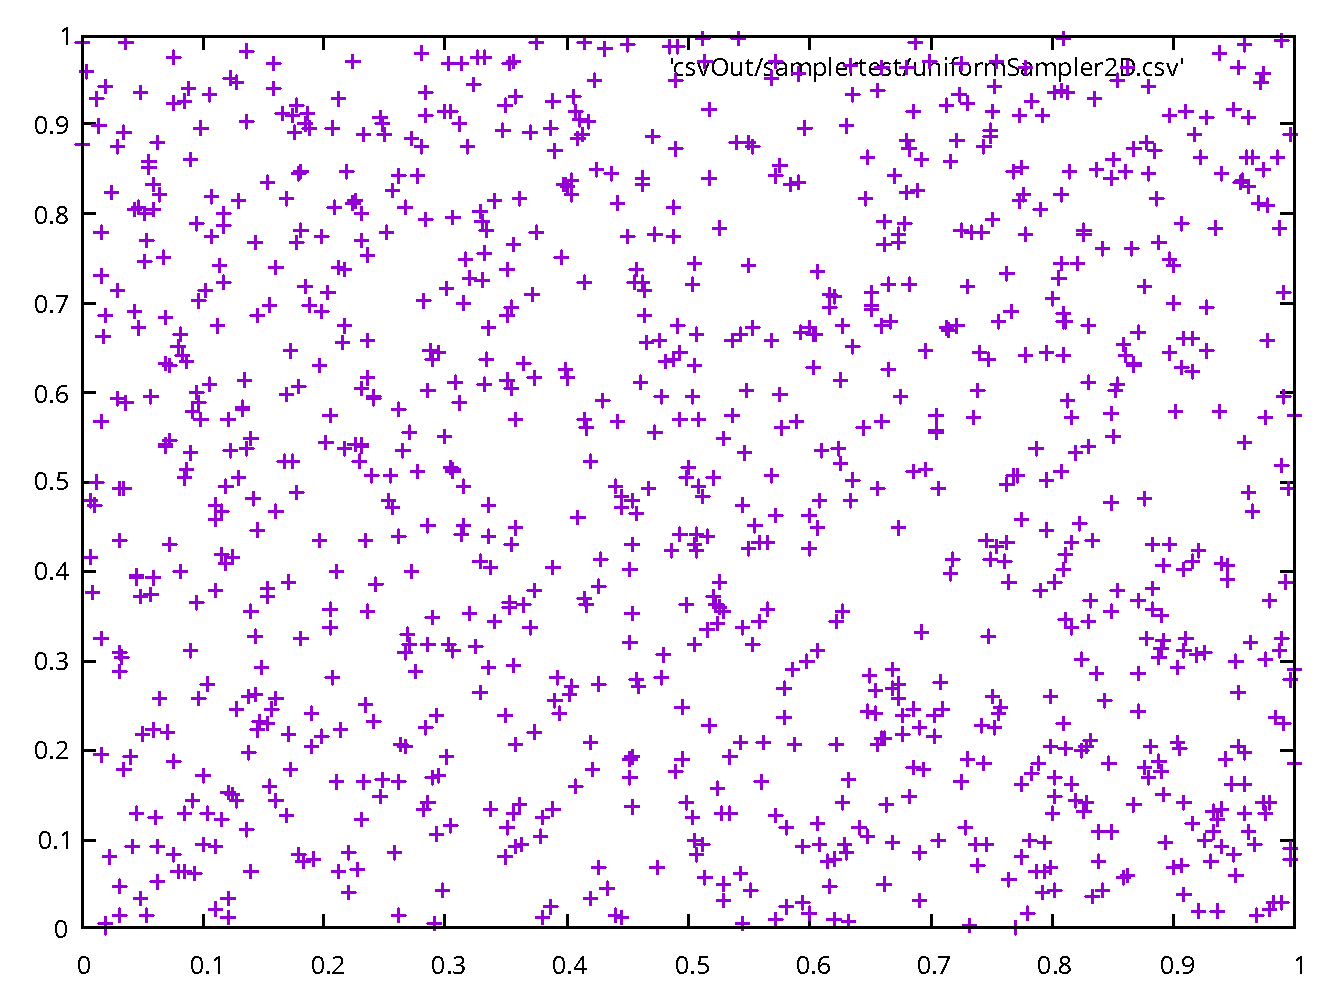
\includegraphics[width=0.5\textwidth]{images/sampling_uniform.pdf} &
            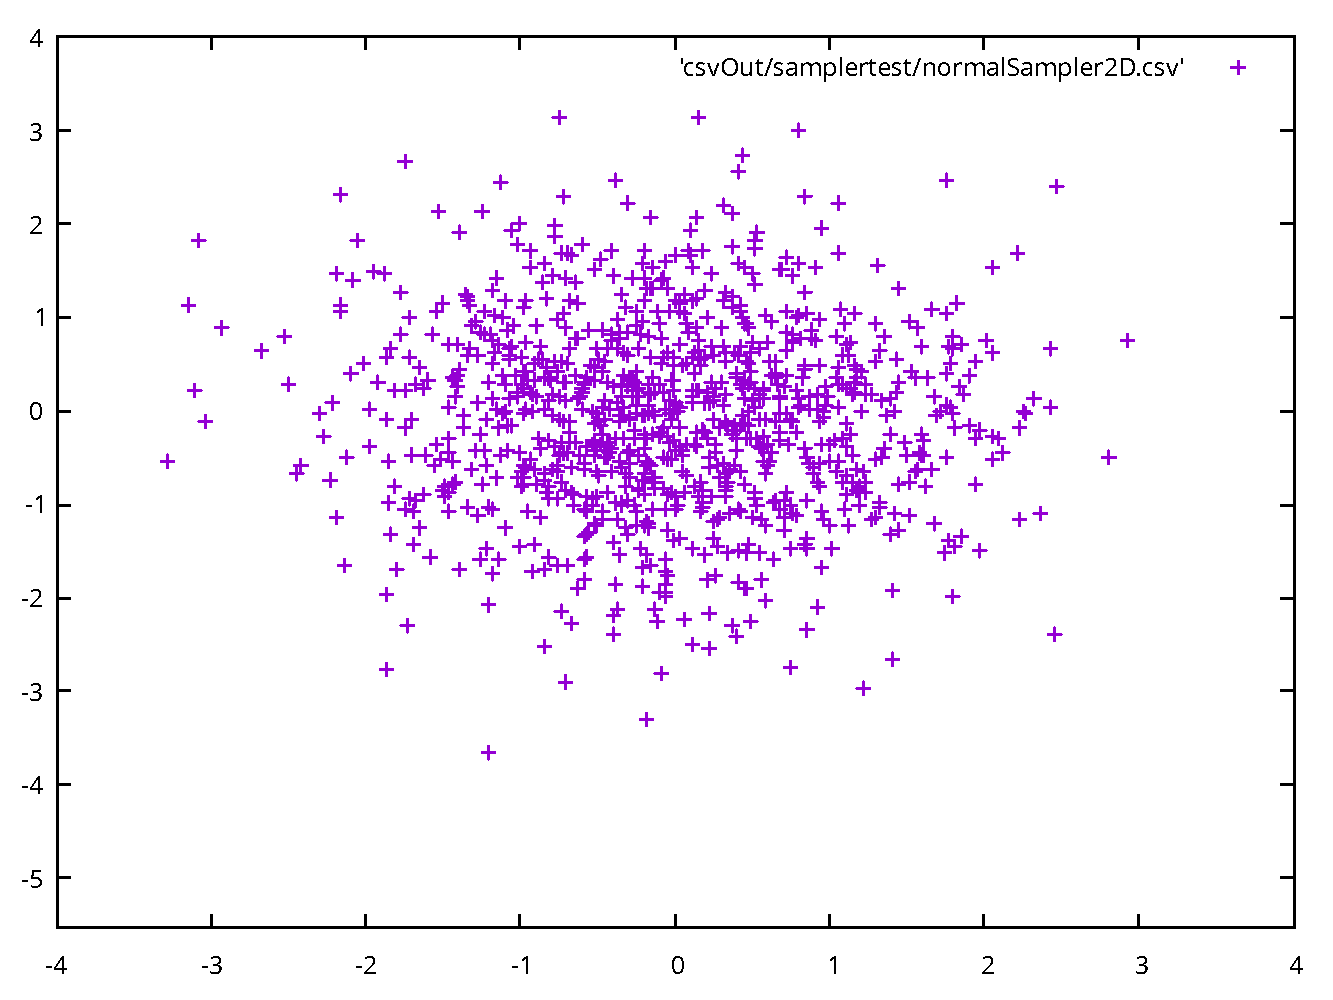
\includegraphics[width=0.5\textwidth]{images/sampling_normal.pdf} \\
            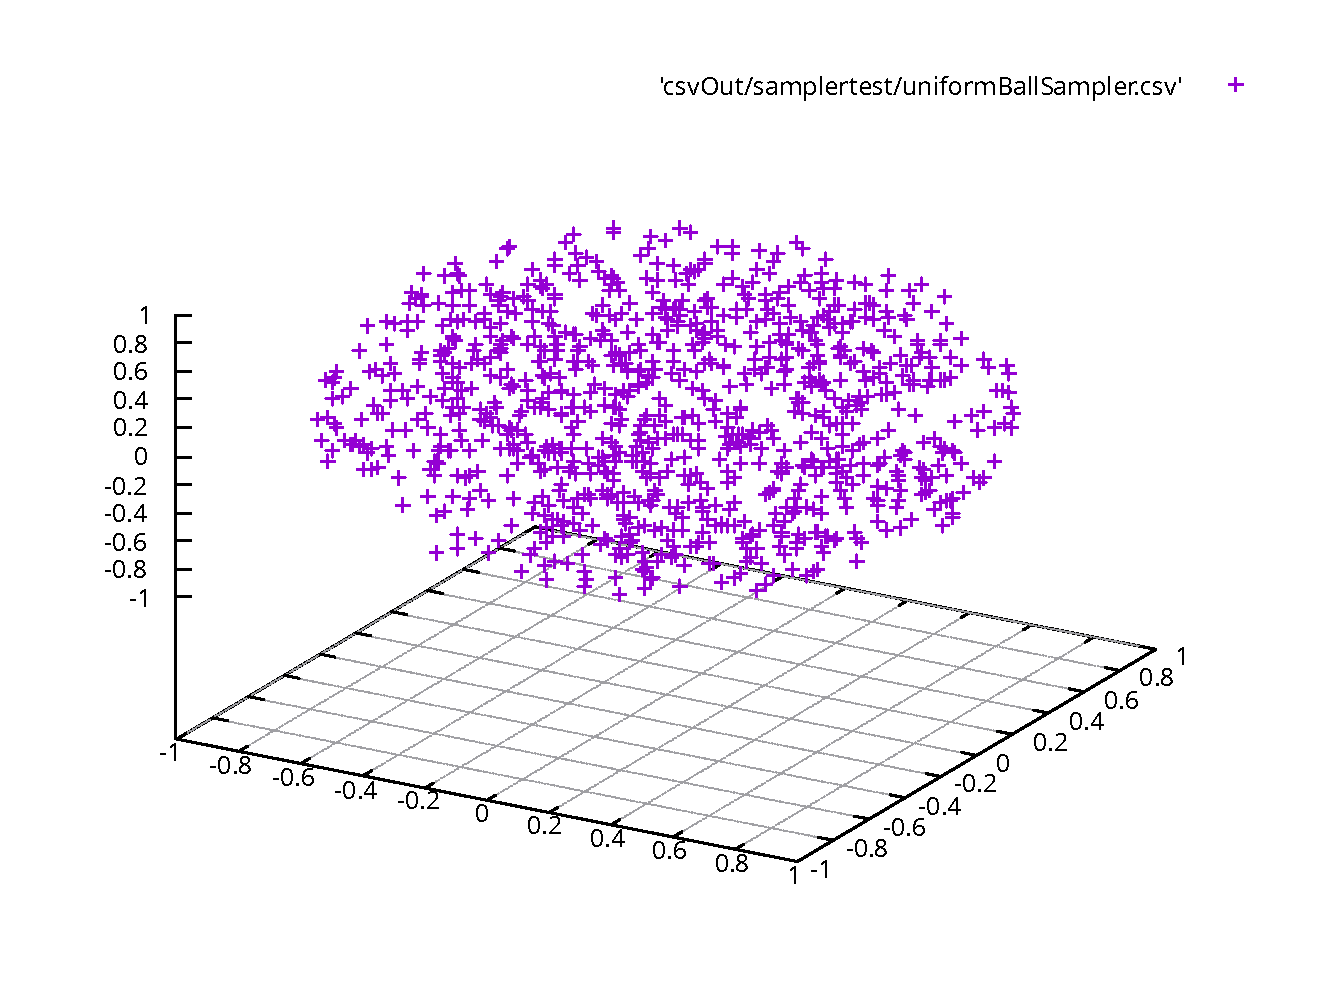
\includegraphics[width=0.5\textwidth]{images/sampling_uniform_ball.pdf} &
            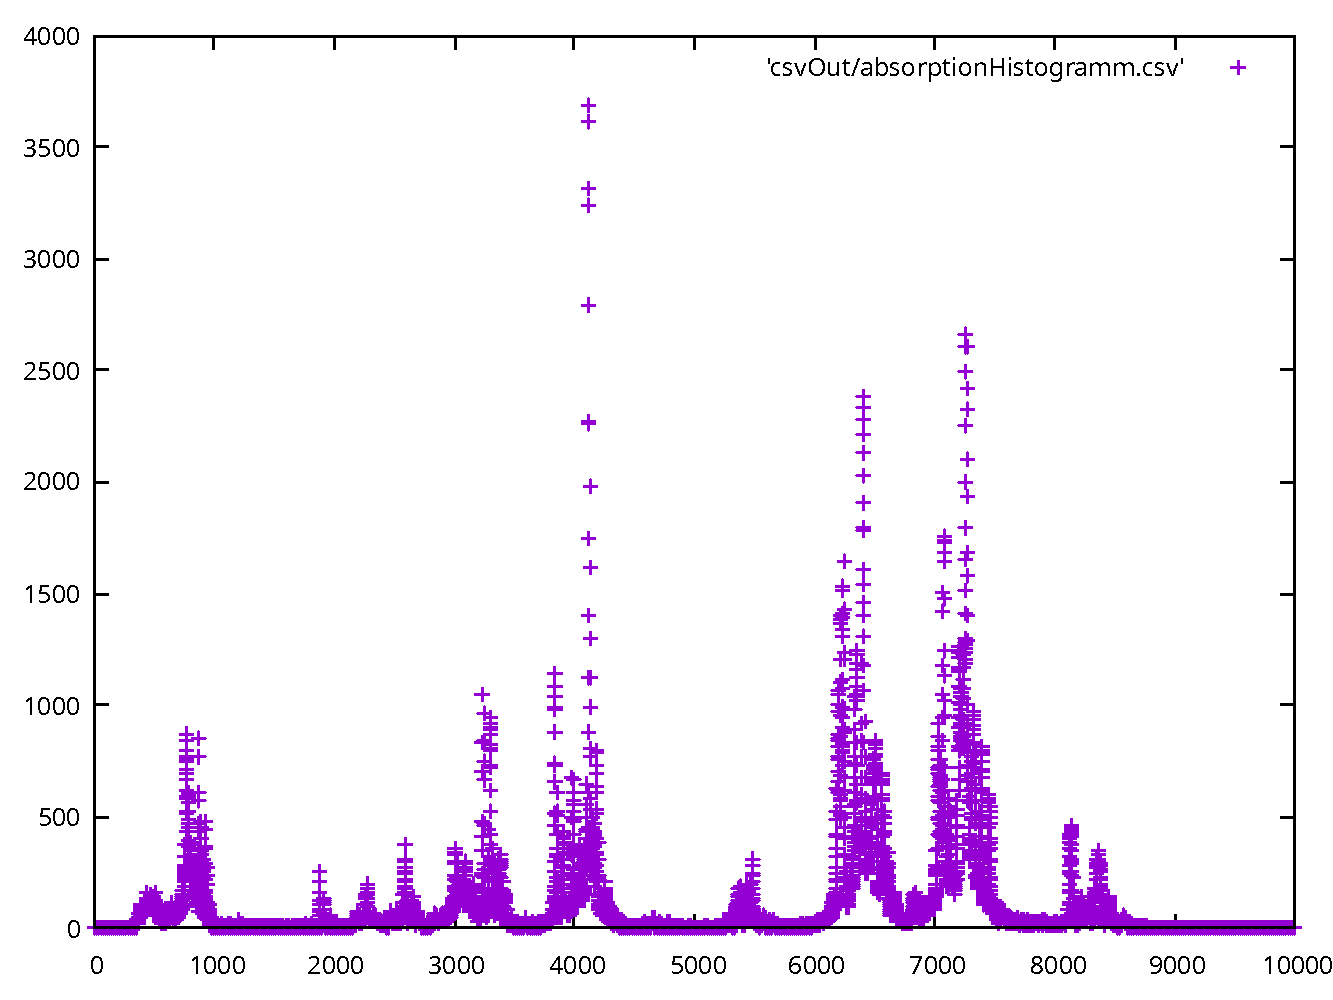
\includegraphics[width=0.5\textwidth]{images/sampling_importance.pdf}
        \end{tabular}
        \caption{
        Different examples of sampler output.
        Two dimensional samplers using the UniformSamplerND (left) and 
        NormalSamplerND (right) classes.
        A three dimensional uniform ball using the UniformBallSampler class
        (bottom left) and a histogramm of an importance sampled distribution
        showing the absorption coefficient for an Nd:YAG crystal (bottom right).
        Higher value means that the respective index has been sampled more often.
        }
        \label{fig:sampler_example}
    \end{figure}
      
    \subsubsection{Utilities} \label{sec:utilities}
    
    \section{Optimization}

    \subsection{Optimization Methods Overview} \label{sec:opt_overview}

    In fields like scientific computing and artificial intelligence
    finding some minimum of a function is a common problem.
    For a given function $f : \mathbb{R}^n \rightarrow \mathbb{R}$ 
    and a domain $\Omega$ the problem is described by 
    \equref{equ:optimization_global}.

    \begin{equation}
        \label{equ:optimization_global}
        \begin{gathered}
        \text{Find} \quad \vec{x}_{min} \in \Omega \subseteq \mathbb{R}^n \quad \text{s.t.}\\
        f(\vec{x}_{min}) \leq f(\vec{x}) \quad \forall \vec{x} \in \Omega
        \end{gathered} 
    \end{equation}

    To solve these kinds of problems a multitude of numerical
    optimization methods are employed.
    Since the applications of numerical optimization are so diverse
    in nature, the functions to optimize often have a wide variety
    of mathematical properties that can be exploited in order to solve
    the problem more quickly or more accurately.
    A general rule for choosing an optimization algorithm for a given
    function, is to use any information available beforehand just by the
    description of the problem.
    For example, one might know that the function's second derivative is
    strictly positive, implying that the shape of the function is convex.
    With this knowledge one can deduct that there is a global minimum, 
    thus the algorithm can be chosen accordingly, and that the 
    solution of this algorithm will be the the global minimum.
    Unfortunately it is often the case that many properties of a 
    physical simulation can only be evaluated using
    complex program codes and cannot be described in a linear or 
    even closed mathematical form and thus produce nonlinear
    dependencies on the input parameters.

    To solve these class of nonlinear optimization problems one employs
    iterative methods that should converge to a solution within a
    finite amount of steps.
    The definition of optimality is also of concern when defining
    what condition actually constitutes a solution.
    In the most cases one wants to find the global minimum as described
    in \equref{equ:optimization_global}.
    Knowing that the minimum which is found by any method is actually
    the global minimum is not possible in general.
    It can be proven mathematically~\cite{solomon_numerical} that it is only possible to know
    for convex functions, but for non-convex
    functions a lesser optimality criterium for local minima has to suffice.
    A modified optimality criterium for non-convex functions is given
    by \equref{equ:optimization_local} where a local minimum is reached
    once the function value is smaller than all other function values 
    in an epsilon ball $B_{\epsilon}$ around the minimum.

    \begin{equation}
        \label{equ:optimization_local}
        \begin{gathered}
        \text{Find} \quad \vec{x}_{min} \in \Omega \subseteq \mathbb{R}^n \quad \text{s.t.}\\
        f(\vec{x}_{min}) \leq f(\vec{x}) \quad \forall \vec{x} \in B_{\epsilon}(\vec{x}_{min})
        \end{gathered} 
    \end{equation}

    Depending on the knowledge about the function $f$, one has to choose
    between a large number of iterative methods.
    Iterative methods can be roughly categorized into second-order, 
    first-order and zero-order optimization algortihms.
    The second-order algortihms rely on the second derivative or
    Hessian matrix of the function to converge.
    First-order methods evaluate the gradient of the function, whereas
    zero-order methods only need to evaluate the function itself.
    As stated before, neither of these categories is better or worse
    per se but depending on the problem at hand some algorithms
    may perform better than others.
    "Better" in this context can also mean completely different things
    depending on the use case.
    In a microcontroller controlling the flightpath of a rocket
    time constraints may be significantly more important than
    scientific calculations running in a laboratory analysis.
    The main difference of the three types of categories is accuracy
    and time constraints.
    The Newton method~\cite{solomon_numerical} - a second-order method -
    chooses the stepsize after eveluating the steepest descent
    direction optimally using the Hessian matrix, thus needing
    a fewer amount of steps and delivering an accurate solution to
    the problem.
    But on the other hand if one does not have the second derivative
    in a closed form already,
    computing the Hessian matrix needs $O(N^2)$
    function evaluations, whereas the gradient descent method
    - a first-order method - only needs to evaluate the gradient, which
    takes the order of $O(N)$ function evaluations.
    As a tradeoff the stepsize in the gradient descent method is not
    known and can be chosen too large, in this case constantly
    overshooting the solution and never satisfying the stop
    criterium, or it can be chosen too small, needing a lot of
    unnecessary iteration steps to finally reach the solution.
    
    Unlike the optimization of well posed analytical problems, scientific
    simulations are often hard to analyze in terms of slope and 
    curvature, and often produce non-smooth noisy results.
    Disregarding the noise, some problems might even be smooth and
    differentiable for a certain neighborhood of values but non smooth
    for others.
    To identify these neighborhoods is in itself a non trivial problem,
    that might involve a large amount of computational expense.
    Especially for codes that rely on some sort of random number generation
    the goal is often to generate some sampled version of the actual function
    that is represented at random sample points, so the whole
    objective is to gradually "uncover" an unknown function where
    little about the expected result is known beforehand.
    These types of functions are often called \emph{oracle} functions
    or \emph{black-box} functions, implying that properties like
    the slope or curvature are either not well defined at some points
    or are not available to the optimization algorithm.
    This situation can occurr in a variety of applications and
    for a variety of reasons.
    One reason might be that a small there are some points where the
    black-box function is non-smooth and therefore not differentiable.
    So an optimization algorithm that evaluates the gradient directly
    at those points will deliver incorrect results or will
    not be stable.
    Another reason can be that the black-box function might be
    computationally expensive to evaluate at a single point making
    the calculation of a gradient or even just part of the gradient
    infeasable in an iterative context.
    So the goal in this case would be to optimize a function with
    a minimal amount of actual function evaluations.
    For these cases of application zero-order or derivative-free 
    optimization has enjoyed increasing popularity in recent years.

    \subsection{Derivative-Free Optimization} \label{sec:derivative_free}

    As discussed in \secref{sec:opt_overview} derivative-free 
    optimization does not rely on the gradient as information for
    the stepping scheme.
    This has the advantage that the number of function evaluations
    is low compared to first-order or second-order methods.
    Of course this is only the case if the derivatives have to be
    calculated numerically.
    If the derivatives are given in a closed form then one generally
    should use first or second-order methods, as these methods
    usually exploit this knowledge in some way to get results
    either faster or more accurately.
    But if the derivative is not given in a closed form but has to be
    calculated by evaluating a series of expensive fuction calls, then
    derivative-free methods can shine.

    As stated by Larson, Menickelly and Wild in~\cite{derivative_free_methods},
    "Derivative-free optimization methods are sometimes employed for 
    convenience rather than by necessity".
    Keeping the strengths and weaknesses of derivate free optimization
    methods in mind, there always most be a justification to use
    a certain method.
    In this work a ray tracing simulation provides a function value
    (or multiple) depending on some geometric parameters of the 
    simulation setup.
    There are three major reasons why it was decided to use derivative
    free approaches to optimize those geometric parameters.
    The first reason is that there are configurations in the
    simulation setup where the function value is discontinuous.
    This can be seen in \figref{fig:opt_discontinuous} where a two
    dimensional domain was evaluated quite densely to make the discontinuous
    parts visible.
    Of course this cannot be done during the optimization algorithm, 
    because it would take a lot of computational cost to just evaluate
    the whole domain.
    To sample the function as densely as in \figref{fig:opt_discontinuous}
    in hihger dimensions one would have to sample exponentially many
    more points depending on the dimensions.

    \begin{figure}
        \centering
        \begin{tabular}{c}
        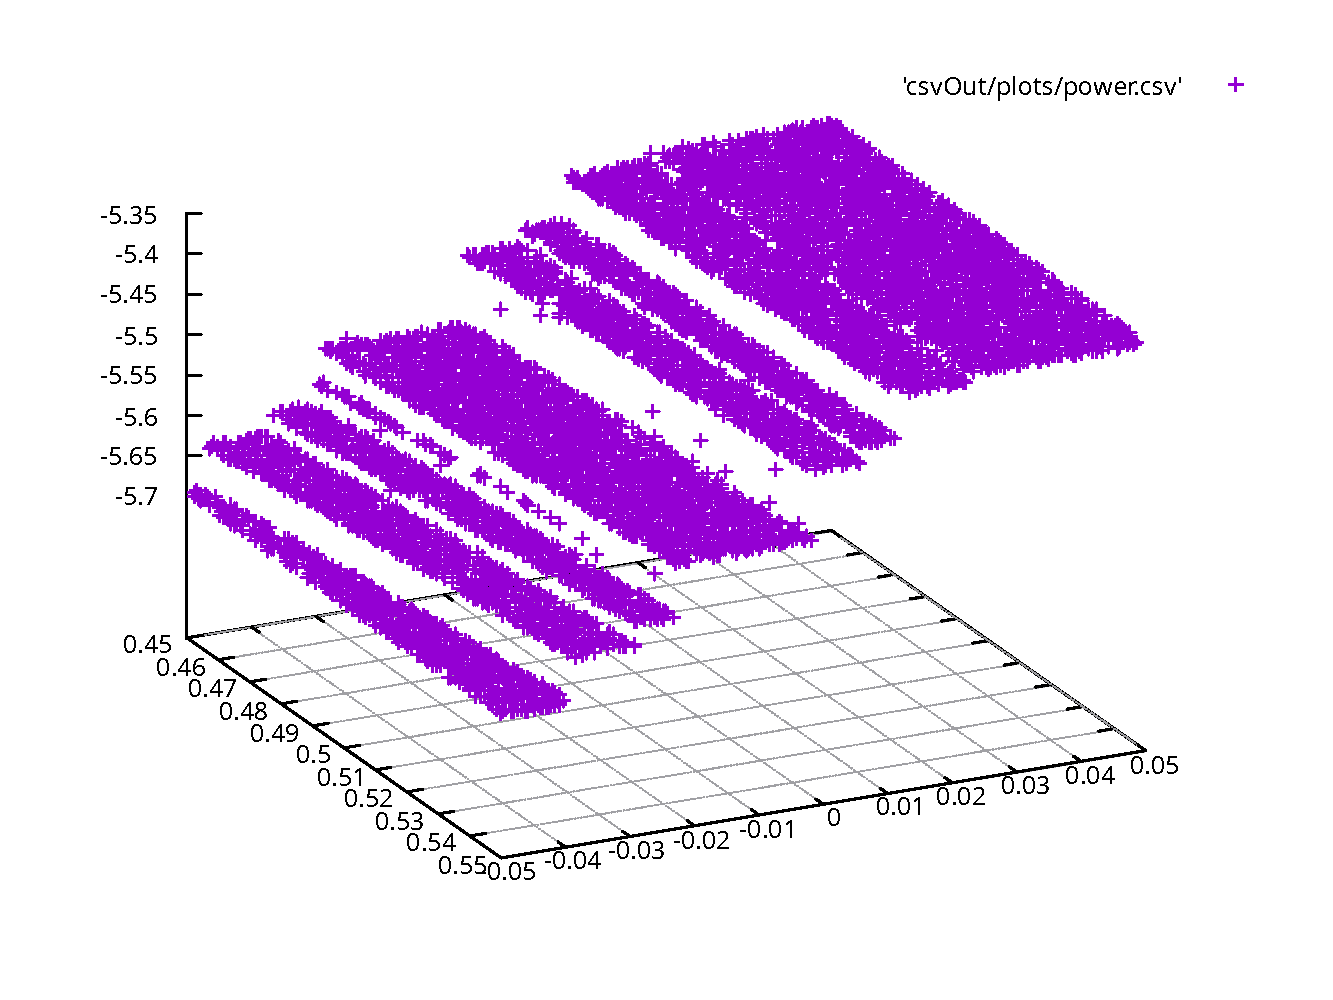
\includegraphics[width=0.8\textwidth]{images/discontinuity.pdf} \\
        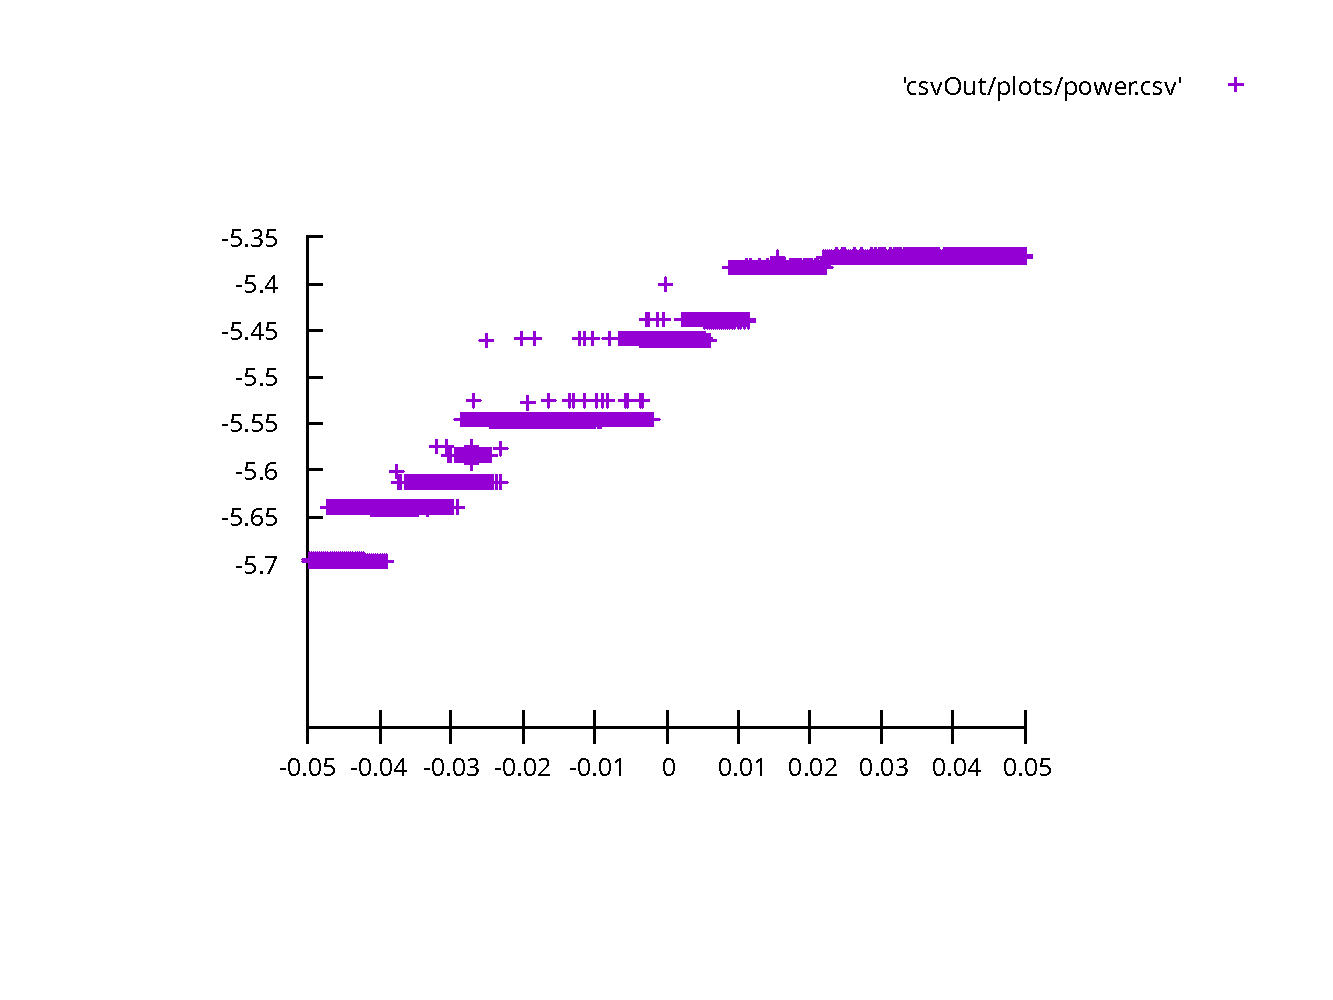
\includegraphics[width=0.8\textwidth]{images/noisyness.pdf}
        \end{tabular}
        \caption{
            Discontinuous (top) and noisy (bottom) points of an objective function
            resulting from a ray tracing simulation.
            The bottom plot is just the same plot as the top one but rotated
            to make the noisy points more visible.
            The simulation was carried out using a similar setup to the setup described
            in \secref{sec:setup} but with a parabolic mirror of the form
            $a*x^2 + b$ where $a$ and $b$ are would be the two input
            parametes to the optimization algorithm.
            It can be observed that the objective function is more a stepfunction than
            a continuous one, making the calculation of a gradient using
            finite differences inpractical.
            Additionally, one can observe that the function has deterministic noise 
            on top of the discontinuity.
        }
        \label{fig:opt_discontinuous}
    \end{figure}

    Another reason why it was chosen to use derivative free optimization
    is the computational cost associated with evaluating the function.
    One evaluation amounts to an entire raytracing simulation of the
    scene using a significant amount of rays and detail in the scene
    to achieve low noise.
    As most derivative free algorithms are specifically designed to
    minimize the amount of function evaluations, this is the
    main reason why a black box optimization algorithm was chosen.
    Especially since the simulation is intended to be uses with multiple
    dimensions of free parameters, each additional dimension would
    cost a lot in terms of gradient evaluation.
    Even more so if one calculates the second-order gradient using
    central differences.
    The thid reason is that derivative free optimization methods
    can deal well with noisy input.
    This is particularly useful if the function is evaluated
    with some sort of random sampling involved.
    In this work the ray tracer calculates the absorption of light in a
    transmissable medium.
    The geometry, power, and wavelength of the rays in the scene are
    randomly sampled.
    This means that across multiple evaluations of the function the
    result varies slightly due to noise generated by the random sampling.
    This is a common problem in raytracing and can only be reduced by
    sampling more often, i.e. shooting more rays into the scene.
    Since the computational cost has to be limited for a function
    evalution in some capacity the noise level cannot be reduced
    to zero completely.
    It is to be noted though that during the simulation all
    random variables are kept the same and the sampling only
    occurs during the setup process of the simulation.
    Thus two evaluations of the function with the same parameters
    deliver the same result.
    This means that there is noise but the noise is deterministic
    in nature.
    Evaluating a gradient with noisy values is generally a bad idea
    and will lead to large variance in the direction in the 
    calculated gradient.
    One could resort to just averaging the gradient across a
    larger domain of points in order to smoothen the noise.
    While this is certainly possible it comes with even more
    computational cost than just calculating the gradient normally.
    Additionally, there is no easy why to calculate a gradient
    analyticly.
    It is technically possible to generate an algorithmic
    differentiation as an alternative to derivative free 
    methods as discussed in ~\cite{derivative_free_methods}.
    The idea here is to generate a derivative by evaluating the
    written code and applying the chain rule for differentiation
    for the elementary operations the code executes.
    This can work well for simple codes and codes without a
    significant amount of absolute values and conditional jumps.
    But after considering that raytracing basically consists of
    trigonometric functions, absolute values and conditional jumps
    it was deemed inpractical to try an approach with algorithmic
    differentiation.
    For these reasons gradient based and therefore also second-order
    methods along with algortihmic differentiation was not used in
    this work and derivative free methods were preferred instead.

    There are also multiple types and categories of derivative
    free optimization.
    These split into two general types.
    Deterministic methods are methods where the decision process of
    the algorithm only depends on information gathered and not
    as in randomized methods also on some factor of randomness
    introduced by a random variable.
    These types of optimization then also depend on whether the
    black-box function is itself deterministic or has stochastic
    elements to it.
    As described above, in this work the black-box function is
    noisy but the evaluation is stricly deterministic.
    Therefore here only methods are explained where the function
    is deterministic.
    Perhaps confusingly one can still aplly randomized methods on
    a deterministic function.
    This can have the benefit of not getting stuck on stationary
    saddle points as easily as deterministic methods.
    In fact most presented methods can be extended to use some
    factor of randomization and thus becoming randomized
    methods.
    Also there are hybrid methods which use some parts of
    each subtype making the distinction between methods not
    as clear.
    As in this work the deterministic MADS algorithm is used on
    a deterministic but noisy function, only
    deterministic methods relevant to the understanding of
    MADS are explained.
    
    The first family of deterministic methods are direct search methods of which
    the later used MADS~\cite{mads_original} algorithm is also a 
    part of.
    Direct methods do not attempt to approximate some sort of gradient
    and generally evaluate a selection of points in order to advance
    towards a minimum.
    These are split into simplex methods and directional direct
    search methods.
    
    Simplex methods use a simplex vertex structure and a set
    of operations on those vertices to iteratively advance the vertices
    to a local minimum.
    The most well known of which is the Nelder-Mead method, where
    the vertex with the biggest function value is continuously
    reflected through a hyperplane spanned by the other points.
    The simplex can also be expanded, contracted or shrunk depending
    on the value of the function at the vertex points.
    It has been shown that the Nelder-Mead method has some drawbacks
    and convergence of the method to a stationary point is not always
    guaranteed~\cite{derivative_free_methods}.
    For this reason simplex methods where ruled out for the optimization
    of the problem presented in this work.
    
    The directional direct search methods always have a current point
    $\vec{x_k}$ and a set of poll points generated by some set
    of directions $\vec{d} \in D_k$ and a current step size $\alpha_k$
    ~\cite{derivative_free_methods}.
    The function is then evaluated at those poll points and the 
    point with the smallest value becomes the new search point 
    $\vec{x_{k+1}}$.
    If there was no poll point with a smaller value the step
    size $\alpha_k$ is decreased and a new set of poll points is
    evaluated.
    It is to be noted that across multiple iterations the set of
    directions can change from one iteration to the next.
    A general algorithm for direct search methods was given in
    ~\cite{derivative_free_methods} as Algorithm 1 and 2 and 
    an abbreviated version is 
    repeated here for the sake of putting the used MADS
    algorithm explained in ~\cite{mads_original} and 
    \secref{sec:mads} in this work into better context. 

    \begin{algorithm}
        \label{alg:direct_search}
        \SetAlgoLined
        Set $0 < \gamma_{dec} < 1 \leq \gamma_{inc}$ \\
        Set initial point $\vec{x}_0$ \\

        \For{$k$ in 0,1,2,...}
        {
            Choose a finite set of search points $Y_k$ \\
            \For{$\vec{y}$ in $Y_k$}{
                $searchpoints \leftarrow f(\vec{y})$ 
            }
            Choose best $\vec{x}_k^p$ from $searchpoints$ \\
            \If{$\vec{x}_k^p = \vec{x}_k$}{
            \For{$\vec{d}$ in $D_k$}{
                $pollpoints \leftarrow f(\vec{x} + \alpha_k \vec{d})$ 
            }
            Choose best $\vec{x}_k^p$ from $pollpoints$ \\
            }
            \If{$\vec{x}_k^p = \vec{x}_k$}{
                $\alpha_{k+1} \leftarrow \gamma_{dec} \alpha_k$
            }
            \Else{
                $\alpha_{k+1} \leftarrow \gamma_{inc} \alpha_k$
            }
            $\vec{x}_{k+1} \leftarrow \vec{x}_{k}^p$
        }
        
        \caption{
            A general direct search algorithm for derivative free
            optimization taken and abbreviated from 
            ~\cite{derivative_free_methods}.
        }
    \end{algorithm}

    Note that before evaluating the poll points a search step can
    be executed, where the function can be sampled at some
    points in hopes to find a better local minimum.
    This step is optional and can potentially help improve the 
    performance of the algorithm.
    The different methods of direct search generate the directions
    $D_k$ differently.
    As stated in ~\cite{derivative_free_methods}, convergence
    proofs for directional direct search methods require that the
    set $D_k$ is a so called \emph{positive spanning set} for the
    domain $\Omega$.
    This means nothing more than that the set of directions form
    a spanning set for describing any point $\vec{x}$ in the domain $\Omega$
    using only positive factors.
    Meaning that every $\vec{x}$ can be written as a sum of 
    directions $\vec{d}_i$ and scale factors $\lambda_i \geq 0$ in 
    \equref{equ:pss}.

    \begin{equation}
        \label{equ:pss}
        \vec{x} = \sum_{i=0}^{|D_k|} \lambda_i \vec{d}_i
    \end{equation}

    If the set of directions $D_k$ is a subset of some fixed
    positive spanning set $D$ one calls the derived methods
    \emph{generalized pattern search} methods or GPS in short.
    The original proposal for the MADS algorithm~\cite{mads_original}
    used in this work contrasts the way MADS chooses those directions
    compared GPS methods and highlights the advantage of not being
    limited to a fixed set $D$ of positive spanning directions,
    especially when it comes to handling of black-box constraints
    and convergence analysis.
    This is explained in more detail in \secref{sec:mads}.

    Other than direct search methods there are also model based
    methods.
    Here the black-box function is modelled by surrogate representing
    the function.
    When iterating the function is locally approximated by a function
    that has some desireable properties for optimization.
    For example a surrogate function could be a polynomial
    which is known to be smooth and differentiable.
    The optimization is then carried out by using information
    the surrogate function provides.
    As usually the model is not accurate across the entire domain,
    but only locally around the current search point.
    The decision if a step should be taken is also influenced
    by an estimation of the error the model has at that point.
    Methods that use this information to make decisions are called
    derivative-free trust-region methods.
    Once the model has been formed around the current search point
    the gradient of the model has to be evaluated.
    This now is possible in a closed form as the mathematical description
    and properties of the model function is known.
    So the main problem with gradient based methods is circumvented
    by this approach.
    One drawback is the relyance on the smoothness of the model function.
    While the model function is smooth the original black-box
    function can be highly discontinuous.
    Thus the model is either not trusted at the discontinuous points
    or a larger number of points needs to be evaluated in order to
    "model" the discontinuity.
    These methods work well if the model function can closely resemble
    the original function.
    This is a problem in the simulation carried out in this work, since
    the objective function is discontinuous and noisy.
    
    In conlusion it was determined that derivative free direct search
    methods offer the most suitable features for the task at hand.
    In particular one special form of direct search called the
    mesh adaptive direct search (MADS) offers the capacity to
    deal with the non smoothness and noisyness of the objective
    function in this work.
    Additionally it can handle constraints on the input parameters
    even if they are also given in a black-box or oracle form,
    something that can come in handy in the design process of 
    any optical system.
    The MADS algorithm can work with a limited amount of black-box
    evaluations and prohibits the unnecessary evaluation of
    the objective function at points that do not satisfy constraints.
    This is benefitial in the design phase of optical systems as
    often manufacturing limitations need to be considered when
    optimizing certain parameters. 
    Furthermore it offers the capability of solving biobjective
    optimization, which is also required when opimizing both
    the absorbed power and the variance of the absorption profile.
    The MADS algorithm is explained and examined in detail in 
    \secref{sec:mads}.
    
    \subsection{Mesh Adaptive Direct Search (MADS)} \label{sec:mads}

    The mesh adaptive direct search class of algorithms was originally
    proposed by Audet and Dennis in 2006~\cite{mads_original}.
    It was specifically designed to optimize nonlinear, nonsmooth
    constrained functions.
    The explanations in this chapter are taken from~\cite{mads_original}
    and theoretical mathematical concepts for the purpose of understanding
    the inner workings of MADS are added where deemed necessary.

    \subsubsection{Optimality and Clarke's Calculus for nonsmooth Optimization} 
    \label{sec:optimality}

    Usually optimality in an optimization problem of the form as in
    \equref{equ:optimization_local} is defined by the notion of stationary
    points.
    A stationary point is a point where the gradient goes to 0 in all
    directions ~\cite{solomon_numerical}.
    Therefore a stationary point $\vec{x}$ must satisfy \equref{equ:stationary_grad}.

    \begin{equation}
        \label{equ:stationary_grad}
        \nabla f(\vec{x}) = 0
    \end{equation}

    For most cases this criterium is adequate if the function $f$ is differentiable.
    Since the direct directional search methods where mainly developed
    to optimize non-smooth functions, one needs a more general way
    of defining optimiality.
    Defining optimality in a different way implies that a substitute
    definition of the derivative or differentiability as a whole
    is required.
    There are many ways of defining some sort of generalized derivative.
    One way of defining a generalized gradient is described by Clarke
    in ~\cite{clarke}.
    Here Clarke proposes a gradient which consists of a set of vectors
    rather than a single vector.
    To understand Clarke's definition, a few mathematical definitions
    and explanations are needed beforehand.
    
    \begin{definition}
        \label{def:local_lipschitz}
        Let $X$ be a Banach space.
        A real valued function $f$ is locally Lipschitz continuous in $\vec{x}$
        if for every $\vec{x} \in X$ exists a neighborhood $N_x$ and a Lipschitz
        constant $K_x$ s.t. for every $\vec{y}, \vec{z} \in N_x$ holds 
        \begin{equation}
            |f(\vec{y}) - f(\vec{z})| < K_x|y - z|
        \end{equation}

        A function $f$ is called locally Lipschitz continuous if it is
        locally Lipschitz continuous for every $\vec{x} \in X$.
    \end{definition}
    
    \defref{def:local_lipschitz} is just a restriction of Lipschitz continuity
    to a neighborhood around a point.
    Lipschitz continuity basically says that the function is continuous in
    that point and the slope of the function is bounded by the constant $K_x$.     
    Lipschitz continuity in that sense is even stronger than continuity
    since additionally to normal continuity the slope has to be bounded.

    \begin{definition}
        Let $\{a_n\} \subset \mathbb{R}$.
        \begin{equation}
            \lim_{n \rightarrow \infty} \sup a_n = \lim_{n \rightarrow \infty} A_n
        \end{equation} 
        where
        \begin{equation}
            A_n = \sup\{a_n, a_{n+1}, ...\} = \sup\{a_k | k \geq n\}
        \end{equation}
    \end{definition}

    The limit superior of a series $a_n$ is just the limit of a series, which consists
    of the smallest upper bounds for a modified series, which
    starts at increasingly later points in the original series.
    One can think of a value that is the smallest possible value that is
    an upper bound of a series (function values) at $n \rightarrow \infty$.
    So basically ome is not interested in the bounding values in the start
    of the series but in the bound which eventually is a bound for all
    values except for a finite amount of values. 
    With those definitions Clark defined the generalized directional
    derivative as in \defref{def:generalized_deriv}.

    \begin{definition}
        \label{def:generalized_deriv}
        Let $X$ be Banach, $\vec{v} \in X$ some direction and 
        $f : X \rightarrow \mathbb{R}$ a real valued
        function that is locally Lipschitz continuous.
        The generalized directional derivative or Clarke directional
        derivative of $f$ at $\vec{x}$ in direction $\vec{v}$ is given by

        \begin{equation}
            f^{\circ}(\vec{x};\vec{v}) = 
            \lim_{y \rightarrow x; \lambda \downarrow 0} \sup
             \frac{f(\vec{y} + \lambda \vec{v}) - f(\vec{y})}{\lambda}
        \end{equation}

    \end{definition}

    The Clarke directional derivative represents an upper bound for the
    slope in direction $\vec{v}$ as one gets closer and closer to $\vec{x}$.
    This is useful since at some point the slope is definitely bound
    because of local Lipschitz continuity of $f$.
    It guarantees that the Clarke directional derivative always exists
    for locally Lipschitz contiuous functions and the value of $f^{\circ}$
    is a finite quantity ~\cite{clarke}.
    Colloquially one could say that if one knows that the function always
    has some neighborhood around the current point where the slope is bounded,
    the slope in a certain direction can be defined as the slope
    one finds as one takes infinitely many samples of the slope at
    closer and closer points to the current point, where one wants
    to find the slope.
    This slope then is steeper than almost all sampled points - almost
    all in the mathematical sense means except for a finite amount of
    points - and it is finite.
    This circumvents the problem of a derivative defined only with
    the differential quotient, as those can become infinite or
    undefined if the function does not behave well at $\vec{x}$.
    Clark then defines a gradient from the diectional derivative as
    a set of directions $\xi$, where the projection of $\xi$ onto
    the direction $\vec{v}$ is smaller than the directional
    derivatives for every direction possible.
    
    \begin{definition}
        The Clarke generalized gradient of $f$ at $\vec{x}$ is
        \begin{equation}
            \partial f(\vec{x}) = 
            \{\xi \in X : f^{\circ}(\vec{x}; \vec{v}) >
             \langle \vec{\xi}, \vec{v} \rangle\}
             \quad \forall \vec{v} \in X
        \end{equation}
    \end{definition}

    This definition of a gradient is not used in the algorithm itself
    but is helpful to understand why the algorithm converges even
    for nonsmooth functions.
    It can be proven that for differentiable functions the Clark
    generalized gradient collapses to a set with a single element,
    that being the conventional gradient $\nabla f(\vec{x})$
    ~\cite{mads_original}.
    If function is optimized using GPS methods 
    that produce $\vec{\hat{x}}$ as a solution for the minimum,
    it has been shown by Audet and Dennis as stated in~\cite{mads_original}
    that the conventional gradient is 0 if the function is
    differentiable in $\vec{\hat{x}}$.
    In particular a stationary point as in \equref{equ:stationary_grad}
    was reached.
    But for only locally Lipschitz continuous functions it was shown
    in a convergence analysis by Audet and Dennis that the Clarke 
    generalized directional
    derivatives are nonnegative for the finite set of fixed directions
    used in GPS methods.
    If the criterium for optimality is just the statement that the
    Clarke generalized directional derivatives have to be nonnegative
    along the pattern directions, then GPS methods can provide
    adequate solutions.
    But this restriction to the finite set of directions produces a 
    weaker optimality criterium than the one fullfilled by the
    MADS class of algorithms.
    The criterium for optimality for MADS methods is thus given by
    reaching a Clarke stationary point and is defined in 
    \defref{def:stationary_clarke}.
    
    \begin{definition}
        \label{def:stationary_clarke}
        A point $\vec{\hat{x}}$ is called a Clarke stationary point,
        if the following holds
        
        \begin{equation}
            f^{\circ}(\vec{\hat{x}}; \vec{v}) \geq 0 \quad \forall
             \vec{v} \in \mathbb{R}^n
            \Longleftrightarrow
            0 \in \partial f(\vec{\hat{x}})
        \end{equation}
    \end{definition}

    This definition also neatly showcases a more intuitive way of thinking
    about the Clarks generalized gradient.
    One can think of the set of vectors in the gradient as the directions
    populating a tangent cone limited by the corresponding Clarke directional
    derivatives at that point.
    If the cone has a positive slope on all sides, the point is a minimum.
    Therefore the new formulation of the optimization problem for
    the MADS class of optimization algolrithms is just given by finding
    a Clarke stationary point within the domain $\Omega$.
    Of course for this to happen one would need to sample infinitely
    many directions, which is not possible in the optimization
    algorithm.
    But as with optimization strategies using the normal 
    definition of stationary points in \equref{equ:stationary_grad} it
    is enough to come asymptotically close to fulfilling the
    criterium.
    Whereas in practice one terminates an iterative algorithm using
    normal gradients when the length of the gradient is small
    enough - usually below some threshold $\epsilon$ - it can
    also be said for the MADS class of algorithms that it is
    enough that the directions are asymptotically densely
    sampled.
    Meaning that there is no inherent restriction of which direction
    can be chosen by the algorithm and enough directions have been sampled
    to say the criterium has been fulfilled with a certain degree of
    confidence. 

    \subsubsection{Constrained Optimization with the Barrier Approach}

    Another advantage that MADS algolrithms have is the handling of
    constraints.
    For this it is necessary to revisit the definition of the optimization
    problem once again.
    Constraints usually have to have a special form for most algorithms.
    Either they need to be linear, bounded, or differentiable and so on.
    For the constrained optimization with MADS algorithms none of
    those properties are required.
    The constraints can just be given as black-box functions or
    oracles which decide whether an point satisfies the constraint
    or not.
    A big limitation of GPS methods is the directional dependence of
    evaluating constraint functions caused by the restriction of the poll
    directions to finitely many fixed directions.
    In MADS algorithms the black-box constraints $c_i$ are included to arrive
    at the updated version of the optimization problem in
    \equref{equ:optimality_mads}.

    \begin{equation}
    \label{equ:optimality_mads}
        \begin{gathered}
        \text{Find} \quad \vec{x}_{min} \in \Omega \subseteq \mathbb{R}^n \quad \text{s.t.}\\
        f_{\Omega}^{\circ}(\vec{x}_{min}; \vec{v}) \geq 0 \quad \forall
             \vec{v} \in \mathbb{R}^n
            \Longleftrightarrow
            0 \in \partial f_{\Omega}(\vec{x}_{min})\\
        \text{where} \quad \Omega = \left \{  \vec{x} \vert  c_i(\vec{x}) > 0 \quad \forall \, c_i \right \}\\
        \text{and} \quad f_{\Omega}(\vec{x}) = 
        \begin{cases}
            f(\vec{x}) & \quad \vec{x} \in \Omega \\
            \infty & \quad \vec{x} \notin \Omega \\
        \end{cases}
        \end{gathered}
    \end{equation}

    The MADS class of algorithms can use a so called barrier approach where the
    constraint functions are just treated as points where the objective function
    goes to infinity.
    This is possible, because there is asymptotically dense polling of directions
    so the barriers are accurately found during the iteration.
    The optimization is then carried out as if the domain is unconstrained.
    It is important to note that the barries $\delta\Omega$ are not 
    eveluated beforehand but are only found during the iteration by
    sampling the poll directions and finding those points.
    The points where one or more of the constraints is not satisfied are often called
    infeasable points.
    As stated in ~\cite{mads_original}, "a key advantage of the barrier
    approach is that one can avoid expensive function calls to $f$ whenever
    a constraint is violated".
    This translates to only evaluating the poll directions where the
    poll point is a feasable point.
    The definition of Clarke's directional derivative can then be modified
    so that only feasable points are present in the formula.
    This is modification was originated by Jahn and is also shown
    and referenced in ~\cite{mads_original}.
    Since the modification is quite trivial the definition of optimality
    using this approach does not change much except that the
    "sampled" points for building the tangent cone have to be feasable
    points.  

    \subsubsection{Mesh Generation and Execution of MADS algorithms}

    As stated in \secref{sec:derivative_free}, the generalized algorithm for
    direct directional search optimization is specialized by
    the concrete implementation in terms of how to choose the set of directions
    $D_k$ in each iteration $k$.
    The same is also true for the MADS algorithm where the special properties
    for optimality shown in \secref{sec:optimality} are only arising due
    to the asymptotically dense evaluation of poll directions.
    To achieve this dense sampling of directions, MADS algorithms generate two 
    sets of meshes around the current point.
    It is important to understand that these meshes only exist conceptually and
    no actual datastructure is needed to store information about the mesh
    other than some parameters and values kept track of during the actual
    iteration.
    One of the meshes is an actual mesh subdividing the domain in a finite amount
    of $n_D$ directions $D$.
    The set $D$, like in GPS methods is a fixed positive spanning set spanning
    $\mathbb{R}^n$ as in \equref{equ:pss}.
    The set $D$ can also be viewed as a $n \times n_D$ matrix and thus the
    mesh is defined by \defref{def:mesh}.

    \begin{definition}
        \label{def:mesh}
        The mesh $M_k$ at iteration $k$ is defined by
        \begin{equation}
            M_k = \bigcup_{\vec{x} \in S_k} 
            \left\{ \vec{x} + \Delta^m_k D \vec{z} \, \vert \, \vec{z}
             \in \mathbb{N}^{n_D} \right\}
        \end{equation}        
        where $\Delta_m^k$ is the mesh size parameter and $S_k$ is the 
        set of already visited points.
    \end{definition}

    This definition of a mesh does not differ from GPS methods yet.
    The distinction comes once the poll directions are chosen from this mesh.
    If a trial point does not satisfy one of the constraints, the value of
    the objective function is just set to infinity without calling $f$ in
    any way.
    It is stated in ~\cite{mads_original} that the constraint functions
    $c_i$ should be ordered according to how expensive the evaluation
    of a constraint oracle is.
    It thus is the responsibility of the user that the cheaper constrained
    should be evaluated first.
    The objective function $f_{\Omega}$ is then evaluated at the trial
    points $\vec{x} \in \Omega$.
    Same as in all directional direct search algorithms the user can
    select a finite set $Y_k$ of search points on the mesh at the
    start of an iteration.
    This has the potential benefit of providing flexibility for the user
    to exploit some problem specific knowledge about the objective
    function.
    The way the user chooses those points does not affect the convergence
    properties of the algortihm since the "lower bound" for convergence
    is given by the poll step.
    If a better point is found during the search step this point becomes
    the new best value, the mesh size parameter $\Delta^m_k$ is increased
    and the iteration is continued.
    If the search step does not yield a better solution then the poll
    step is executed and a better solution is searched with the
    trial points produced by the poll directions.
    Should the poll search also fail and the current solution
    still be the best solution, the mesh size for the next iteration
    $\Delta^m_{k+1}$ is decreased to produce a finer mesh and the
    objective function can generally be evaluated closer and closer
    to the current best point.
    The exact rule for updating the mesh size parameter shown in
    ~\cite{mads_original} and given in \equref{equ:meshsize}, were
    $\tau > 1$ and $w^- \leq -1$ and $w^+ \geq 0$ are user defined
    parameters.

    \begin{equation}
    \label{equ:meshsize}
    \begin{gathered}
    \Delta^m_{k+1} = \tau^{w_k}\Delta^m_k \\
    w_k \in 
    \begin{cases}
        \{ 0,1,\dots,w^+\} &\quad \text{if improved point was found} \\
        \{w^-,w^- + 1,\dots, -1\} &\quad \text{else} \\
    \end{cases}
    \end{gathered}
    \end{equation}

    The difference between MADS and GPS methods is how the algorithms choose
    the trial points in the poll step.
    For GPS methods the trial points have to lie a fixed distance away from
    the current point.
    This distance is $\Delta^m_k$ considering the mesh and means that
    the trial points can only be one "hop" away from the current point.
    This inherently limits the possible poll directions to the fixed finite
    set of directions $D$ given in the generation of the mesh.
    If the selection of trial points is independent of the current mesh
    size, the possible trial point are limited by a so called \emph{frame}.
    The frame is defined by separate poll size parameter $\Delta^p_k$
    which limits the mesh distance at which trial point can be from
    the current point.
    For GPS methods it holds that $\Delta^p_k = \Delta^m_k$.
    The MADS class of algortihms on the other hand does not impose such
    a hard restriction on the frame size.
    Here it must hold that $\Delta^p_k \geq \Delta^m_k$ for all iterations $k$.
    The only additional requirement given to the different size parameters is
    that the mesh size needs to tend towards zero if and only if the 
    poll size also tends to zero with progressive iterations.
    This ensures that the sampling of directions is asymptotically dense
    and the modified definition of optimiality in \equref{equ:optimality_mads}
    can be satisfied. 
    
    The process of generating the MADS frame is described in ~\cite{mads_original}
    and yields a positive spanning set of directions $D_k$ which contrary to
    GPS methods is \underline{not} a subset of $D$.
    The set of poll points $P_k$ is a set of mesh points which are generated
    using a nonnegative integer combination $\vec{d}$ of the directions in $D$
    and the mesh size parameter $\Delta^m_k$.
    The distance of the current best point or also called the \emph{frame center}
    is also bound by a constant times the poll size parameter $\Delta^p_k$.
    This ensures that the pollpoints in the frame still lie on the mesh
    but are limited to a certain distance from the frame center.
    The formal definition of a MADS frame is thus given by \equref{equ:madsframe}.

    \begin{equation}
        \label{equ:madsframe}
        P_k = \{\vec{x}_k + \Delta^m_k \vec{d} \, | \, \vec{d} \in D\} \subset M_k
    \end{equation}

    The distinct advantage of such a frame definition is that during the 
    optimization iteration of the MADS class of algorithms, the mesh size
    parameter can decrease more rapidly than the frame size parameter.
    For a GPS method where those two parameters are always equal the number
    of possibilities for poll directions is finite and fixed.
    Now suppose that the MADS algorithm iterates indefinitly and always
    fails to find a better solution point, meaning that the mesh
    and frame size is successively reduced.
    It is ensured that if $\Delta^p_k \geq \Delta^m_k$ holds for all iterations,
    and the mesh size is reduced more rapidly than the poll size,
    the number of possibilities for the poll directions within the frame tends
    towards infinity, thus producing a dense set of directions in the limit.
    Now if all those poll points still do not deliver a better point
    after a certain threshold of iterations or evaluations one can say
    that in the limit the condition for optimiality using Clarke's
    generalized gradient is fullfilled.
    This is indeed proven in ~\cite{mads_original} and the reader is
    encouraged to look at the proof themselves as it is enough for this
    work to understand the inner workings of the MADS algorithm,
    but keeping the convergence analysis for the reader to discover.   
    A nice visual example of what a MADS iteration looks like compared
    to GPS iterations is also given in ~\cite{mads_original} and is
    also shown here, as the quite theoretical definitions become
    intuitively clear when one understands the mesh and frame adaptation
    visually.
    The example illustrates how a finite set $D$ of mesh directions in
    $\mathbb{R}^2$ can generate an infinite amount of poll directions
    for the MADS algortihm but a finite and fixed amount of directions
    for GPS methods.
    So let the set $D$ be the set of eight directions 
    $\{(d_1,d_2)^T \neq (0,0)^T : d_1,d_2 \in \{-1,0,1\}\}$.
    Note that $D$ is a positive spanning set for $\mathbb{R}^2$.
    There are eight different distinct positive spanning sets 
    consisting of three directions.
    The number three is chosen arbitrarily here and can also be
    upto eight directions but at a minimum three directions are 
    required to generate a positive spanning set $D_k$.
    This is due to the fact that factors $\lambda_i$ for a 
    positive spanning set have to be positive as shown in \equref{equ:pss}.
    So in oreder to reach every point in $\mathbb{R}^2$ one needs at
    least two vectors that would be just a spanning set and 
    one additional direction to have some sort of way to reach
    negative directions.
    Examples of what a GPS and MADS iteration could look like for
    a successful iteration, where a point $\vec{x}_k$ stays the
    best solution for multiple iterations, and
    different mesh and frame parameters are shown in \figref{fig:gps}
    and \figref{fig:mads} respectively.
    As can be seen in \figref{fig:gps} the directions for GPS methods
    are restricted to come from the set $D$, because the mesh parameter
    and the frame parameters are the same for each iteration and
    the only possible trial points lie on the intersection of the 
    edge of the frame with the mesh.
    The frames in the MADS iteration in \figref{fig:mads} shrink at the
    rate $\Delta^p_k = n \sqrt{\Delta^m_k}$ which is slower than
    the rate at which the mesh size parameter is reduced.
    The trial points can then be selected from all the mesh points
    inside the frame.
    In the limit $k \rightarrow \infty$ the amount of possible
    trial points in the frame and therefore directions in $D_k$
    also goes to infinity.
    This achieves the desired effect that the polling directions in
    the MADS class of algorithms is asymptotically dense and therefore
    a Clarke stationary point can be identified.

    \begin{figure}
    \centering
    \import{images/}{gps.pdf_tex}
    \caption{
    Example of GPS frames
    $P_k = \{\vec{x}_k + \Delta^m_k \vec{d} \, | \, \vec{d} \in D_k \}
    = \{p^1, p^2, p^3\}$ for different values $\Delta^m_k = \Delta^p_k$.
    Observe that the possible polling directions are limited to the
    original set $D$ and thus $D_k \subseteq D$.
    The figure was redrawn from Figure 2.1 in~\cite{mads_original}}
    \label{fig:gps}
    \end{figure}

    \begin{figure}
    \centering
    \import{images/}{mads.pdf_tex}
    \caption{
    Example of MADS frames
    $P_k = \{\vec{x}_k + \Delta^m_k \vec{d} \, | \, \vec{d} \in D_k \}
    = \{p^1, p^2, p^3\}$ for different values $\Delta^m_k \leq \Delta^p_k$.
    Observe that the possible polling directions are not limited to the
    original set $D$ and thus $D_k \nsubseteq D$. 
    The number of possible polling directions goes to infinity and
    therefore makes the set of sampled directions asymptotically dense.
    The figure was redrawn from Figure 2.2 in~\cite{mads_original}
    }
    \label{fig:mads}
    \end{figure}

    \subsection{Biobjective MADS}
    \subsubsection{Multiobjective Optimization}

    As discussed in the preceeding sections, the problem of single objective
    nonsmooth optimization can be solved using the MADS algorithm.
    Many optimization problems in scientific computation and engineering
    applications have to consider multiple objectives at the same time.
    The optimization problem in this work for example consists of
    optimizing absorbed power in the laser crystal while at the same
    time keeping a low variance of absorbed power across the crystal.
    A high power absorption alone would generate a powerful output
    beam, but one of low quality, while an even distribution of power
    alone would create a high quality beam, but the beam would be of low
    output power.
    For this reason there is a need to optimize a multiobjective function
    which describes both power and variance objectives.
    The multiobjective optimization problem can be formulated as seen
    in \equref{equ:optimization_multi}.

    \begin{equation}
        \label{equ:optimization_multi}
        \begin{gathered}
        \text{Find} \quad \vec{x}_{opt} \in \Omega \subseteq \mathbb{R}^n \quad \text{s.t.}\\
        F:\mathbb{R}^n \rightarrow \mathbb{R}^p \\ 
        F(\vec{x}_{opt}) = (f_1(\vec{x}_{opt}),f_2(\vec{x}_{opt}),\dots,f_p(\vec{x}_{opt}))\\
        \, \text{is optimal}
        \end{gathered}
    \end{equation}

    Note that in \equref{equ:optimization_multi} the question of optimality is
    specificly left vague as in multiobjective optimization a notion
    of minimum does not make much sense.
    This is because now the objective function is no longer real valued.
    It arises the question of what point $\vec{x}$ is more optimal than
    another point $\vec{y}$.
    One can only somehow compare their vector valued images in $F$ and
    has to decide what is inherently a better output, a worse output or
    as a consequence of vector valued outputs an indifferent output.
    indifferent in this sense means that one cannot say what output
    is better or worse, but the point $\vec{x}$ is better than $\vec{y}$
    in some objective functions $f_i$ while it is worse in others.
    This implies there is always a tradeoff in multiobjective optimization
    and one needs a more fitting definition of what it means
    for a point to be optimal.
    A solution to this problem is the definition of \emph{Pareto dominance},
    which is explained in ~\cite{multiobjective} and the next chapter 
    \secref{sec:pareto}.

    \subsubsection{Pareto Dominance and Pareto Fronts} \label{sec:pareto}
    
    To compare two points in order to determine which point is more
    optimal than the other, there cannot be a total order relation defined
    on the image space of $F$.
    Instead there is a partial order relation called \emph{Pareto dominance}
    relation.
    As shown in ~\cite{multiobjective}, this relation is defined in
    \defref{def:pareto_dominance}.
    
    \begin{definition}
        \label{def:pareto_dominance}
        Let $\vec{u},\vec{v} \in X$ be two points of the multiobjective
        function $F: X \rightarrow Y$.
        \begin{itemize}
            \item $\vec{u} \preceq \vec{v}$ ($\vec{u}$ weakly dominates $\vec{v}$)
            $\Longleftrightarrow f_i(\vec{u}) \leq f_i(\vec{v}) \; \forall i \in \{1,\dots,p\}$   

            \item $\vec{u} \prec \vec{v}$ ($\vec{u}$ dominates $\vec{v}$)
            $\Longleftrightarrow \vec{u} \preceq \vec{v} \; \text{and} \; 
            f_j(\vec{u}) < f_j(\vec{v}) \; \text{for at least one} \; j \in \{1,\dots,p\}$   

            \item $\vec{u} \sim \vec{v}$ ($\vec{u}$ is indifferent to $\vec{v}$)
            $\Longleftrightarrow \; \text{$\vec{u}$ does not dominate $\vec{v}$ and $\vec{v}$
            does not dominate $\vec{u}$}$  
        \end{itemize}
    \end{definition}

    For an image point $F(\vec{x})$ \defref{def:pareto_dominance} thus
    subdivides the image space $Y$ or in this case $\mathbb{R}^p$ into three zones.
    The first zone is the \emph{dominance zone}, which are all the image
    points that dominate $\vec{x}$.
    The \emph{dominated zone} then are all the image points dominated and
    the \emph{indifferent zone} are all the image points indifferent to $\vec{x}$.
    An example of this in $\mathbb{R}^2$ image space can be seen in figure
    \figref{fig:dominance_zones}, which is based on Figure 2.1 in ~\cite{multiobjective}.
   
    \begin{figure}
        \centering
        \missingfigure{dominance zones}
        \caption{}
        \label{fig:dominance_zones}
    \end{figure}

    The definition of Pareto dominance alone is not enough to define optimality
    for multiobjective optimization problems.
    Like in the single objective case, it is not guaranteed that a problem
    has a globally optimal solution.
    For this reason it is necessary to define global and local optimality
    in terms of the Pareto dominance relation.
    A definition of global and local optimality for multiobjective problems
    is given in ~\cite{multiobjective} and here in \defref{def:optimality_multi}.

    \begin{definition}
        \label{def:optimality_multi}
        Let $\vec{x} \in X$ be a point of the multiobjective function $F: X \rightarrow Y$.
        \begin{itemize}
            \item $\vec{x}$ is globally Pareto optimal (just called Pareto optimal) 
            $\Longleftrightarrow$
            There exists no $\vec{y}$ s.t. $\vec{y} \prec \vec{x}$.
            If $\vec{x}$ is Pareto optimal then $F(\vec{x})$ is called
            Pareto efficient.

            \item $\vec{x}$ is locally Pareto optimal $\Longleftrightarrow$
            There exists an $\epsilon, \sigma > 0$ for which the set
            $\{\vec{y} \in B_{\epsilon}(\vec{x}) \cap X \, | \, \vec{y} \prec \vec{x},\, 
            F(\vec{y}) \in B_{\sigma}(F(\vec{x})) \}$ is empty.
            If $\vec{x}$ is locally Pareto optimal then $F(\vec{x})$ is called
            locally Pareto efficient.
        \end{itemize}
    \end{definition}

    An intuitive understanding of Pareto efficiency is that there cannot be another
    point in $X$ where all except at least one objective function $f_j$ of the single objective
    functions $f_i$ are either equal or less than the objective functions at the current point,
    whereas $f_j$ is truly smaller.
    As a geometric interpretation in a two dimensional image space this means
    there cannot be another point where the image point is to the left or down or both.
    This is exactly the meaning of dominance zones in \figref{fig:dominance_zones}.
    An example of Pareto efficient points in $\mathbb{R}^2$ is given in \figref{fig:pareto_front},
    which is based on Figure 2.2 in ~\cite{multiobjective} with additional explanations.
    It can be seen that the search for Pareto efficient points returns a
    set of Pareto optimal points $X_p$, of which the dominance zone is outside the
    image space $Y$.
    The image $Y_p$ of the set $X_p$ of points is called the \emph{Pareto front}.
    
    \begin{figure}
        \centering
        \missingfigure{pareto front}
        \caption{}
        \label{fig:pareto_front}
    \end{figure}
    
    The goal of any multiobjective optimization algortihm should be to deliver
    a set of points which approximates the Pareto front as closely as possible.
    There are multiple was of formulating a multiobjective problem as
    a single objective problem.
    One way would be to weight the single objective functions $f_i$ by a factor
    $w_i \geq 0$ so that $\sum_i w_i = 1$.
    As stated in ~\cite{multiobjective}, any solution to this problem is Pareto
    optimal for the multiobjective problem.
    If one solves the linear weighted problem for different combinations,
    a subset of the Pareto front is generated.
    The disadvantage of this method is that not all points of the pareto front
    can be generated due to the limitation to the linear weighted form.
    Another method would be to define a reference point $\vec{r} \in Y$ and
    minimizing the $q$-norm as in \equref{equ:reference_point}, where
    $1 \leq q \leq \infty$.

    \begin{equation}
        \min_{\vec{x} \in \Omega} || F(\vec{x}) - \vec{r} ||_q
    \end{equation}

    The reference point approach has the advantage that it can theoretically
    reach the entire Pareto front.
    Therefore, solving the reference point problem for different reference point
    produces an approximation of the Pareto front~\cite{multiobjective}.
    The only disadvantage is that if the point is chosen incorrectly
    also non efficient points are generated.
    The general question with the reference point approach is how to
    choose those reference points.
    Along with other approaches of solving the multiobjective optimization
    problem, it is also shown in ~\cite{multiobjective} that a general
    parametrized approach with respect to the reference point has some
    properties necessary for optimality in Clarke's calculus, if the
    parametrization conserves Lipschitz continuity and other properties.
    The parametrized version of the single objective formulation of 
    a multiobjective optimization problem uses the parametrized function
    $\Phi_r$ as a real valued objective and is shown in
    \equref{equ:parametrized}.
    
    \begin{equation}
        \label{equ:parametrized}
        \min_{x \in \Omega} \Psi_r(\vec{x}) \quad \quad \Psi_r(\vec{x}) =
         \Phi_r(f_1(\vec{x}),f_2(\vec{x}),\dots,f_p(\vec{x})) 
    \end{equation}

    Depending on the choice of $\Phi_r$ the Pareto front is approximated
    if one solves this problem for a set of reference points.
    This is proven for a bunch of choices for $\Phi_r$ in ~\cite{multiobjective}
    and the reader is encouraged to convince themselves of this property.
    In the next section the concrete implementation of the BiMADS algorithm
    for the solution of biobjective nonsmooth optimization problems 
    is shortly presented.

    \subsubsection{BiMADS}

    The BiMADS algorithm was originally presented by Audet, Savard and Zghal
    in ~\cite{multiobjective} in 2008.
    It uses the MADS algorithm to solve a series of single objective formulations
    of a biobjective problem with increasingly stringent stopping criteria.
    The idea is to iteratively build a set of non-dominated points that
    approximate the Pareto front.
    The set of non-dominated dominated points $X_{\mathcal{L}}$ is updated
    each time the MADS algorithm runs and keeping all visited trial points that
    are non-dominated by the current set $X_{\mathcal{L}}$ and throwing
    away all dominated points in $X_{\mathcal{L}}$.
    The single objective problem the MADS has to solve each iteration is
    a single objective formulation using the parametrized approach in
    \equref{equ:parametrized}.
    The reference point is chosen beforehand using a process which is later
    described in more detail.
    After the update of $X_{\mathcal{L}}$ the list is ordered in ascending
    order according to the value of $f_1$ and in descending order according 
    to $f_2$.
    This is only possible because the amount of objectives is two.
    The ordering is done in order to easily determine the euclidian distance
    between the images $Y_{\mathcal{L}}$ of $X_{\mathcal{L}}$.
    This is done so the point where the euclidian distance in image space $Y$
    is the largest to its neighboring points $\vec{x}_j$ - note that neighboring here only
    makes sense because of the ordering of set $X_{\mathcal{L}}$ according 
    to the previous discussed relation defined for only two objectives
    $f_1, f_2$ - can be determined and the values of the objectives of
    those neighboring points can be combined to get a new reference point $\vec{r}$
    that surely dominates the chosen point $\vec{x}_j$.
    In short, that BiMADS algorithm choses its reference points in a
    way to minimize the gaps between the Pareto efficient points in $Y_{\mathcal{L}}$.
    This achieves better coverage of the Pareto front.
    The MADS algorithm is then executed for the single objective problem
    with respect to $\vec{r}$ and started from the chosen point $\vec{x}_j$.
    Additionally to choosing the reference point, the algorithm then stores
    a weighting factor for that specific $\vec{x}_j$ in order to achieve
    better coverage and increase the stopping criterium for MADS should
    that point be chosen again.
    Once a reference point $\vec{r}$ was derived from a point $\vec{x}_j$ the
    weighting is increased, which then in turn diminishes that points
    ability to be chosen again in the successing iterations.
    This approach of choosing the reference points gives an even distribution
    of non-dominated points along the Pareto front.
    Since the basic idea of the BiMADS algorithm was explained and is
    sufficient to understand the application of the algorithm in this
    work, the convergence analysis for BiMADS is left to the reader
    to study in ~\cite{multiobjective}.
    A detailed overfew of the BiMADS algorithm is given in \algref{alg:bimads}.

    \begin{algorithm}
        \label{alg:bimads}
        \SetAlgoLined
        Initial MADS run to solve $\min_{\vec{x} \in \Omega} f_1(\vec{x})$ and
        $\min_{\vec{x} \in \Omega} f_2(\vec{x})$ at starting point $\vec{x}_0$ \\

        Set $X_{\mathcal{L}} = {\vec{x}_1, \vec{x}_2,\dots,\vec{x}_J}$ to be an
        ordered list of non-dominated points s.t. $f_1(\vec{x}_1) < \dots < f_1(\vec{x}_J)$
        and $f_2(\vec{x}_1) > \dots > f_2(\vec{x}_J)$ \\

        \While{$\delta_{\hat{j}} > threshold$ OR maximum iterations not reached}
        {
           \If{$J > 2$}{
                $\hat{j} \leftarrow \text{argmax}_{j=2,\dots,J-1} \delta_j = 
                \frac{||F(\vec{x}_j) - F(\vec{x}_{j-1})||^2 +
                ||F(\vec{x}_j) - F(\vec{x}_{j+1})||^2}{w(\vec{x}_j) + 1}$\\
                
                Define reference point $\vec{r} \leftarrow (f_1(\vec{x}_{\hat{j} + 1})
                , f_2(\vec{x}_{\hat{j} - 1}))$
           }
           \If{$J = 2$}{
                $\vec{x}_{\hat{j}} \leftarrow \vec{x}_2$ \\
                $\delta_{\hat{j}} \leftarrow \frac{||F(\vec{x}_2) - F(\vec{x}_{1})||^2}{w(\vec{x}_2) + 1}$\\

                Define reference point $\vec{r} \leftarrow (f_1(\vec{x}_{2})
                , f_2(\vec{x}_{1}))$
           }
           \If{$J = 1$}{
                $\vec{x}_{\hat{j}} \leftarrow \vec{x}_1$ \\
                $\delta_{\hat{j}} \leftarrow \frac{\delta}{w(\vec{x}_{\hat{j}}) + 1}$\\
                Execute MADS from $\vec{x}_{\hat{j}}$ to solve $\min_{x \in \Omega} f_1(\vec{x})$
                and $\min_{x \in \Omega} f_2(\vec{x})$. 
                Terminate MADS when mesh size $\Delta^m$ drops below $O(\delta_{\hat{j}})$.
                \emph{Goto} update step.
           }

           Execute MADS for the single objective formulation $\Phi_r$.
           Terminate MADS when mesh size $\Delta^m$ drops below $O(\delta_{\hat{j}})$
           or a maximum number of objective evaluations is reached.\\

           Update $X_{\mathcal{L}}$ by adding all dominant points from the MADS run and
           removing all dominated points.
           Increase weights $w(\vec{x_{\hat{j}}}) \leftarrow w(\vec{x_{\hat{j}}}) + 1
            \quad \forall \vec{x} \in X_{\mathcal{L}}$
        }
        
        \caption{
            BiMADS algorithm
        }
    \end{algorithm}


    \subsection{NOMAD Library}
    \subsection{Integration into Framework}

    \section{Examplatory Setup} \label{sec:setup}
    \subsection{Setup} 
    \subsection{ASLD Software}
    \subsection{Beam Analysis}

    \newpage

    \bibliographystyle{plain}
    \bibliography{bibliographies/references}

\end{document}
